\chapter{Challenges and Research Goals}
\label{chapter:challenges-and-research-goals}

State of the art in automatic joinery machines and its design-to-production workflows have indicated that the technical bottleneck to prefabricate unique timber parts have long been solved. The entire production workflow from CAD design to joinery fabrication have already been digitised and automated. The next research frontier is to automate the assembly of the components into a complete structure. Using timber frame structures with integral timber joints as a starting target, this thesis aims to explore the roadblocks that are still in the way of automatic spatial timber assembly. The goal is to better understand existing challenges, discover new problems, identify possible solutions, develop new models and pave the way for future in-depth research.

The general research question is ``\textbf{How can robots assemble spatial timber structures?}". However, the formulation of more specific questions is treated as a product of first understanding precedence works and their challenges. This approach allows for a more focused study on the commonly encountered problems and to steer towards generalizable solutions while avoiding common culprits. Therefore, this chapter will start by presenting the known challenges related to the automatic assembly of spatial timber structures before summarising on the more detailed research questions that are pursued in the rest of the thesis. This chapter consists of two parts: 

\textbf{Section 2.1 Mechanical Challenges} focuses on the mechanical tasks that are physically performed during the construction. It represents the fabrication part of the ``Digital Fabrication" paradigm - the automation of the production tasks.

\textbf{Section 2.2 Computation and Design Challenges} presents the computational problems required to prepare the information for the robotic process. In particular, the automatic and human-in-the-loop workflows to create robotic programmes from a design. It represents the digital part of the ``Digital Fabrication" paradigm - the automation of the production of digital information.

Finally, research questions are formulated in \textbf{Section 2.3 Research Questions}. 

\section{Mechanical Challenges}
\label{section:challenges-mechanical-challenges}

\subsection{Sliding Friction}
\label{subsection:challenges-sliding-friction}

During the closure of a timber joint, surfaces between each pair of joints start to make contact. Apart from butt joints\footnote{ Definition of butt joints for this thesis are joints that do not have rubbing contact surfaces. Contact force only appears when the beam reaches its final, assembled position}, most of the joints are designed with a substantial amount of contact surfaces that will slide and rub against each other during assembly. For example (Figure \ref{fig:rubbing-surface-in-lap-during-assembly}) , the amount of rubbing surfaces in a pair of half lap joints increases during assembly. 

\begin{figure}[h]
     \centering
     \begin{subfigure}[b]{0.32\textwidth}
         \centering
         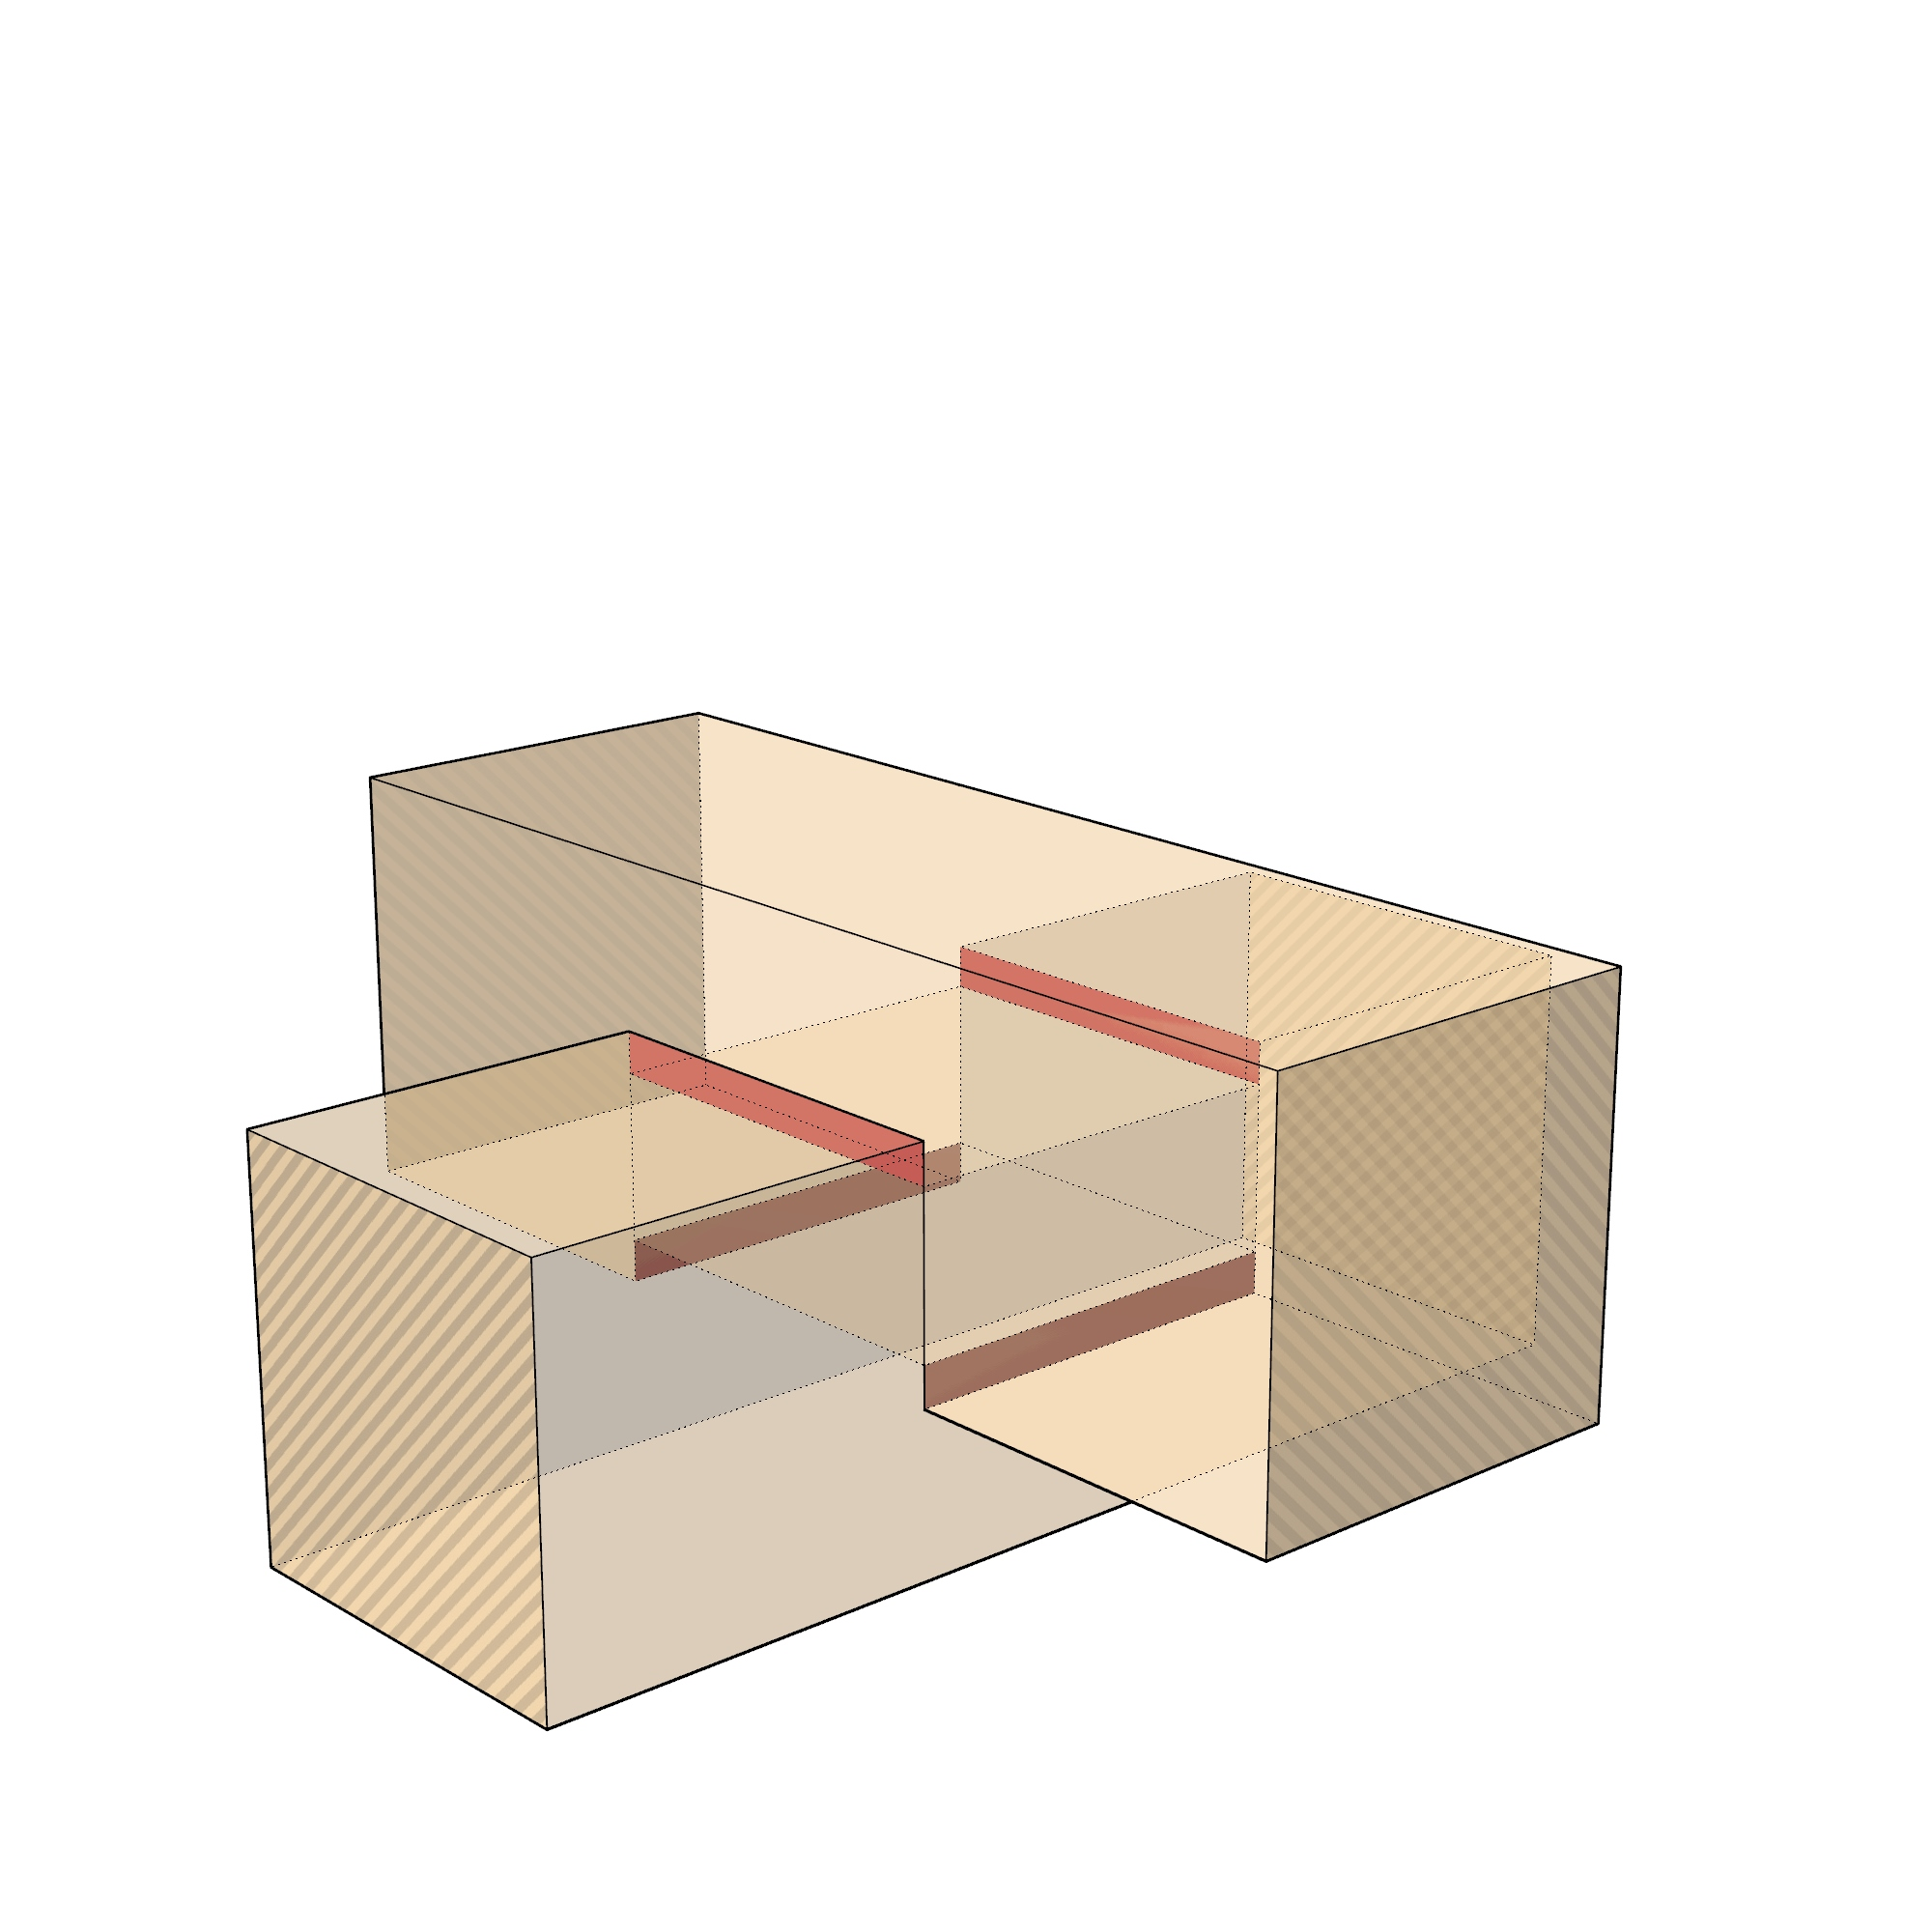
\includegraphics[width=\textwidth]{images/02/LapJoint_4.jpg}
         % \caption{SubFigureCaption}
         %\label{fig:uniquesubfigurelabel}
     \end{subfigure}
     \hfill
     \begin{subfigure}[b]{0.32\textwidth}
         \centering
         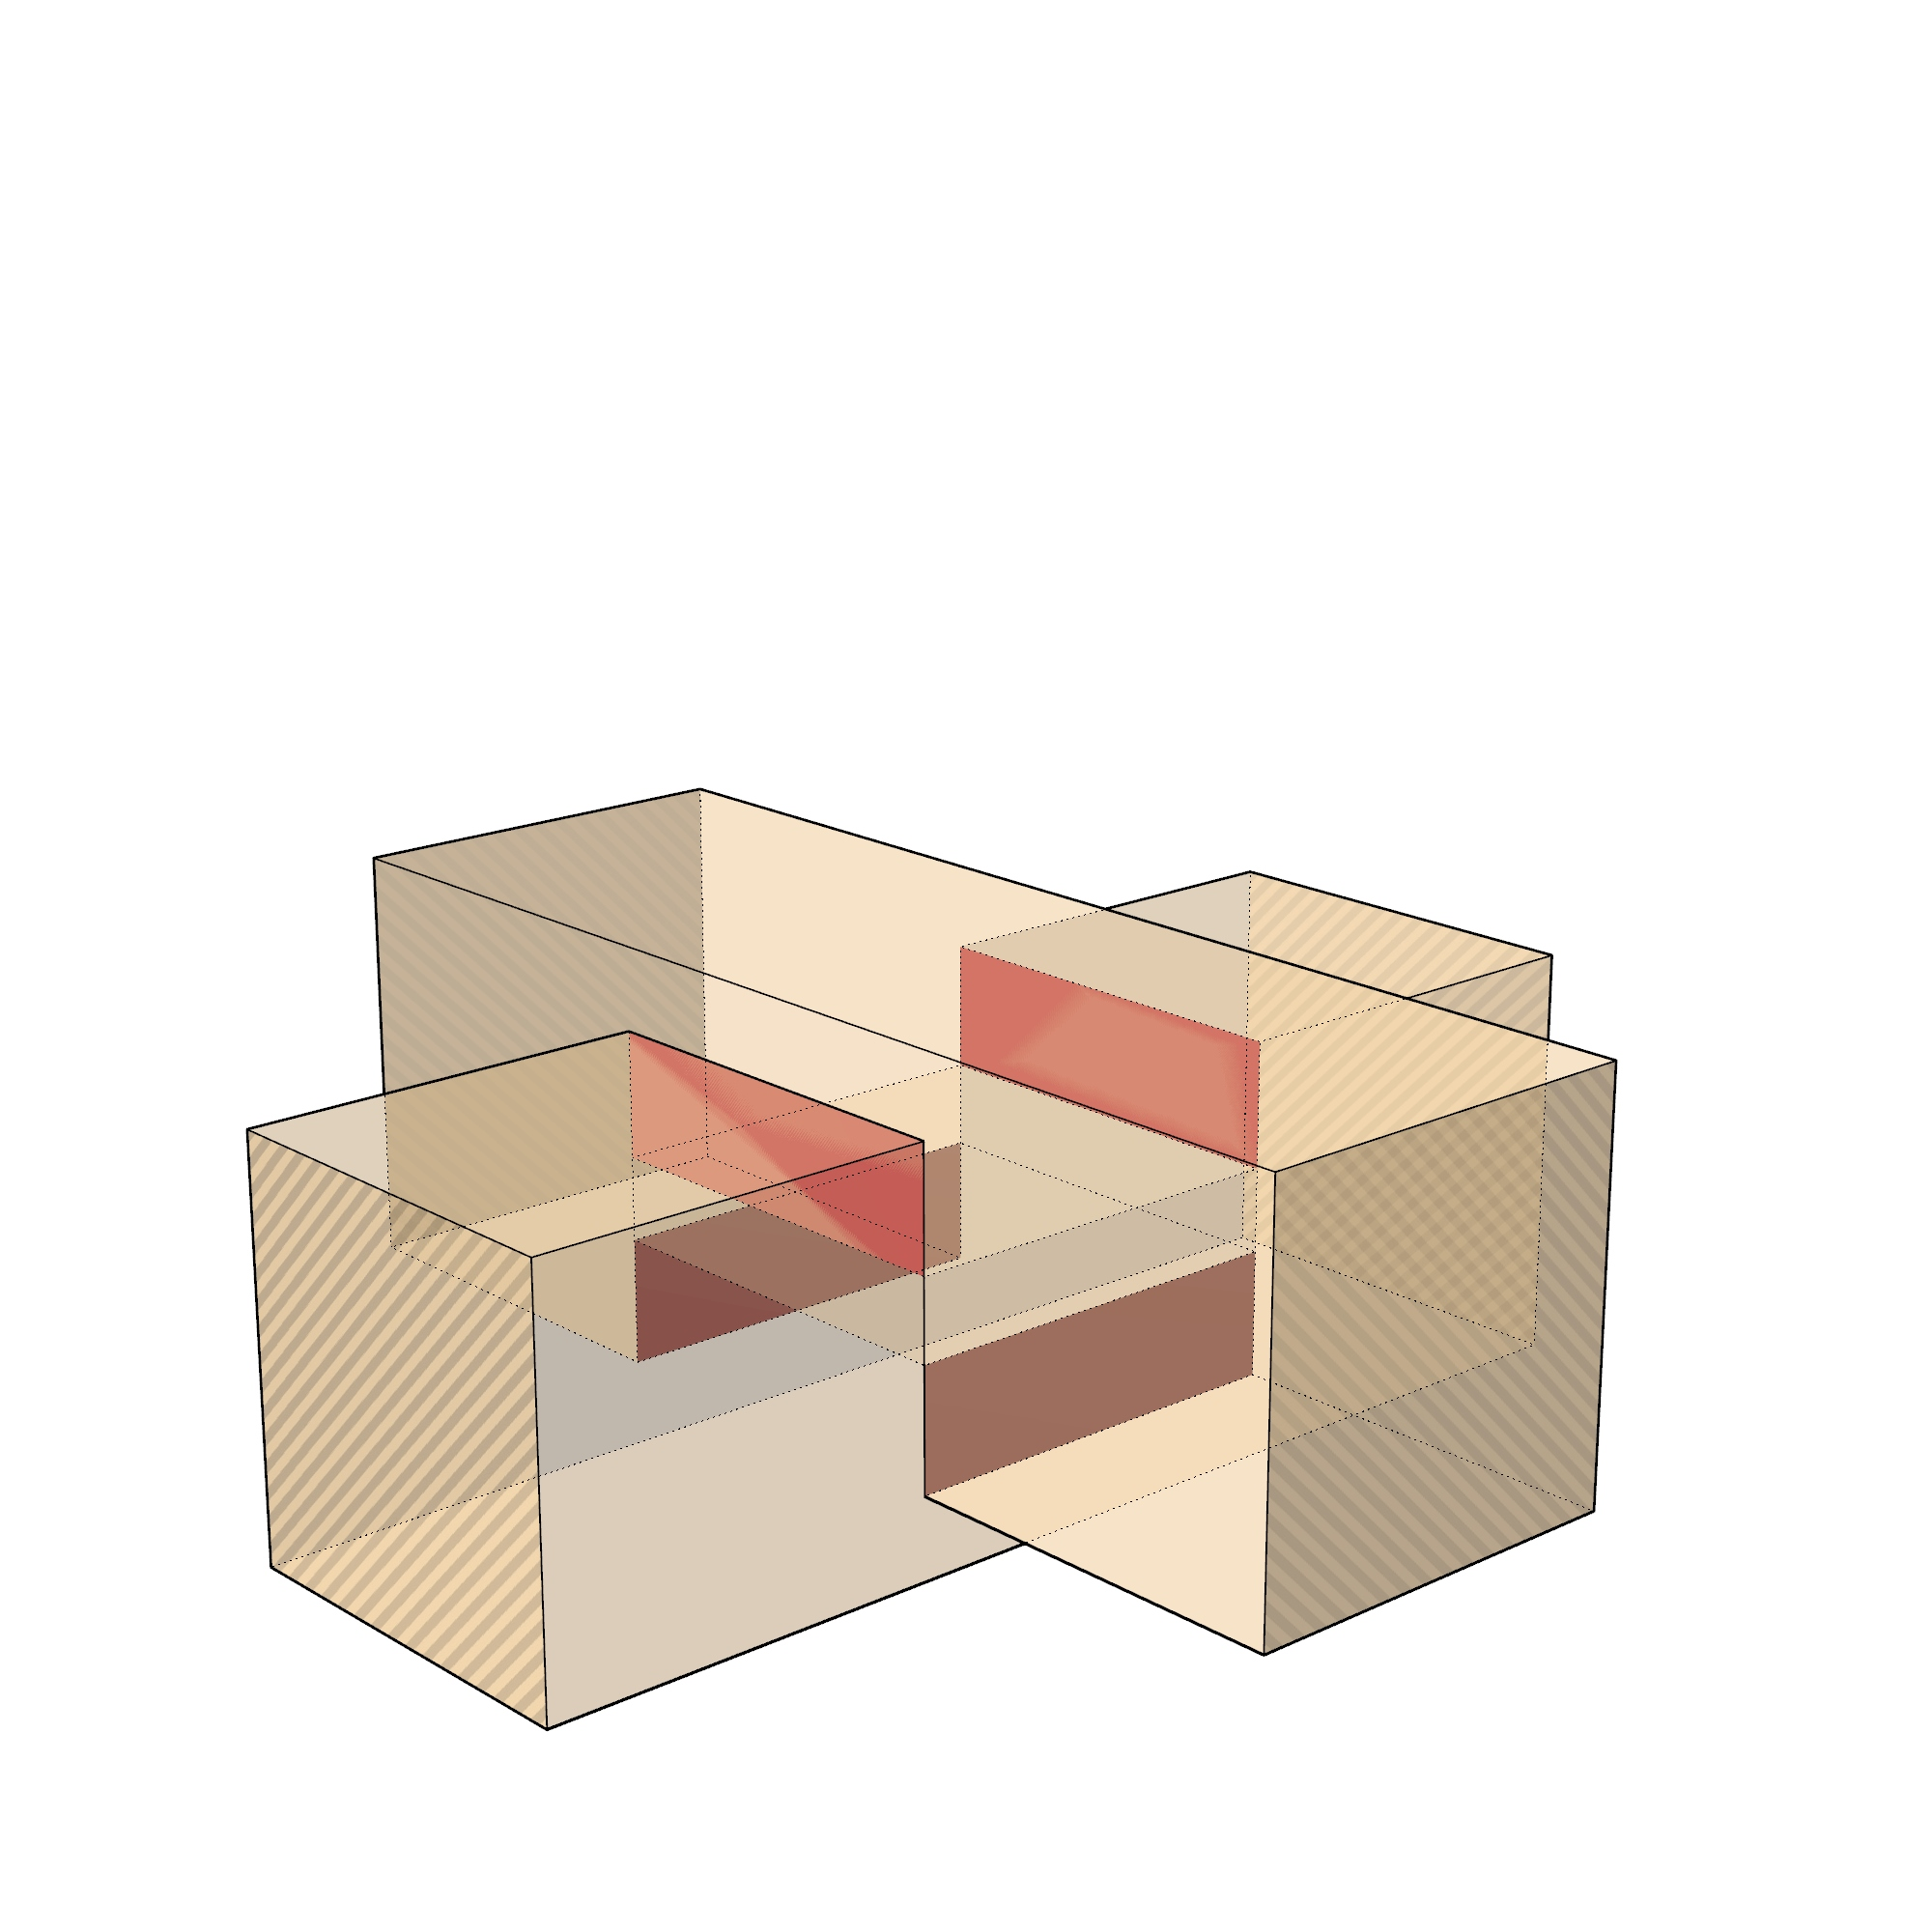
\includegraphics[width=\textwidth]{images/02/LapJoint_5.jpg}
         % \caption{SubFigureCaption}
         %\label{fig:uniquesubfigurelabel}
     \end{subfigure}
     \hfill
     \begin{subfigure}[b]{0.32\textwidth}
         \centering
         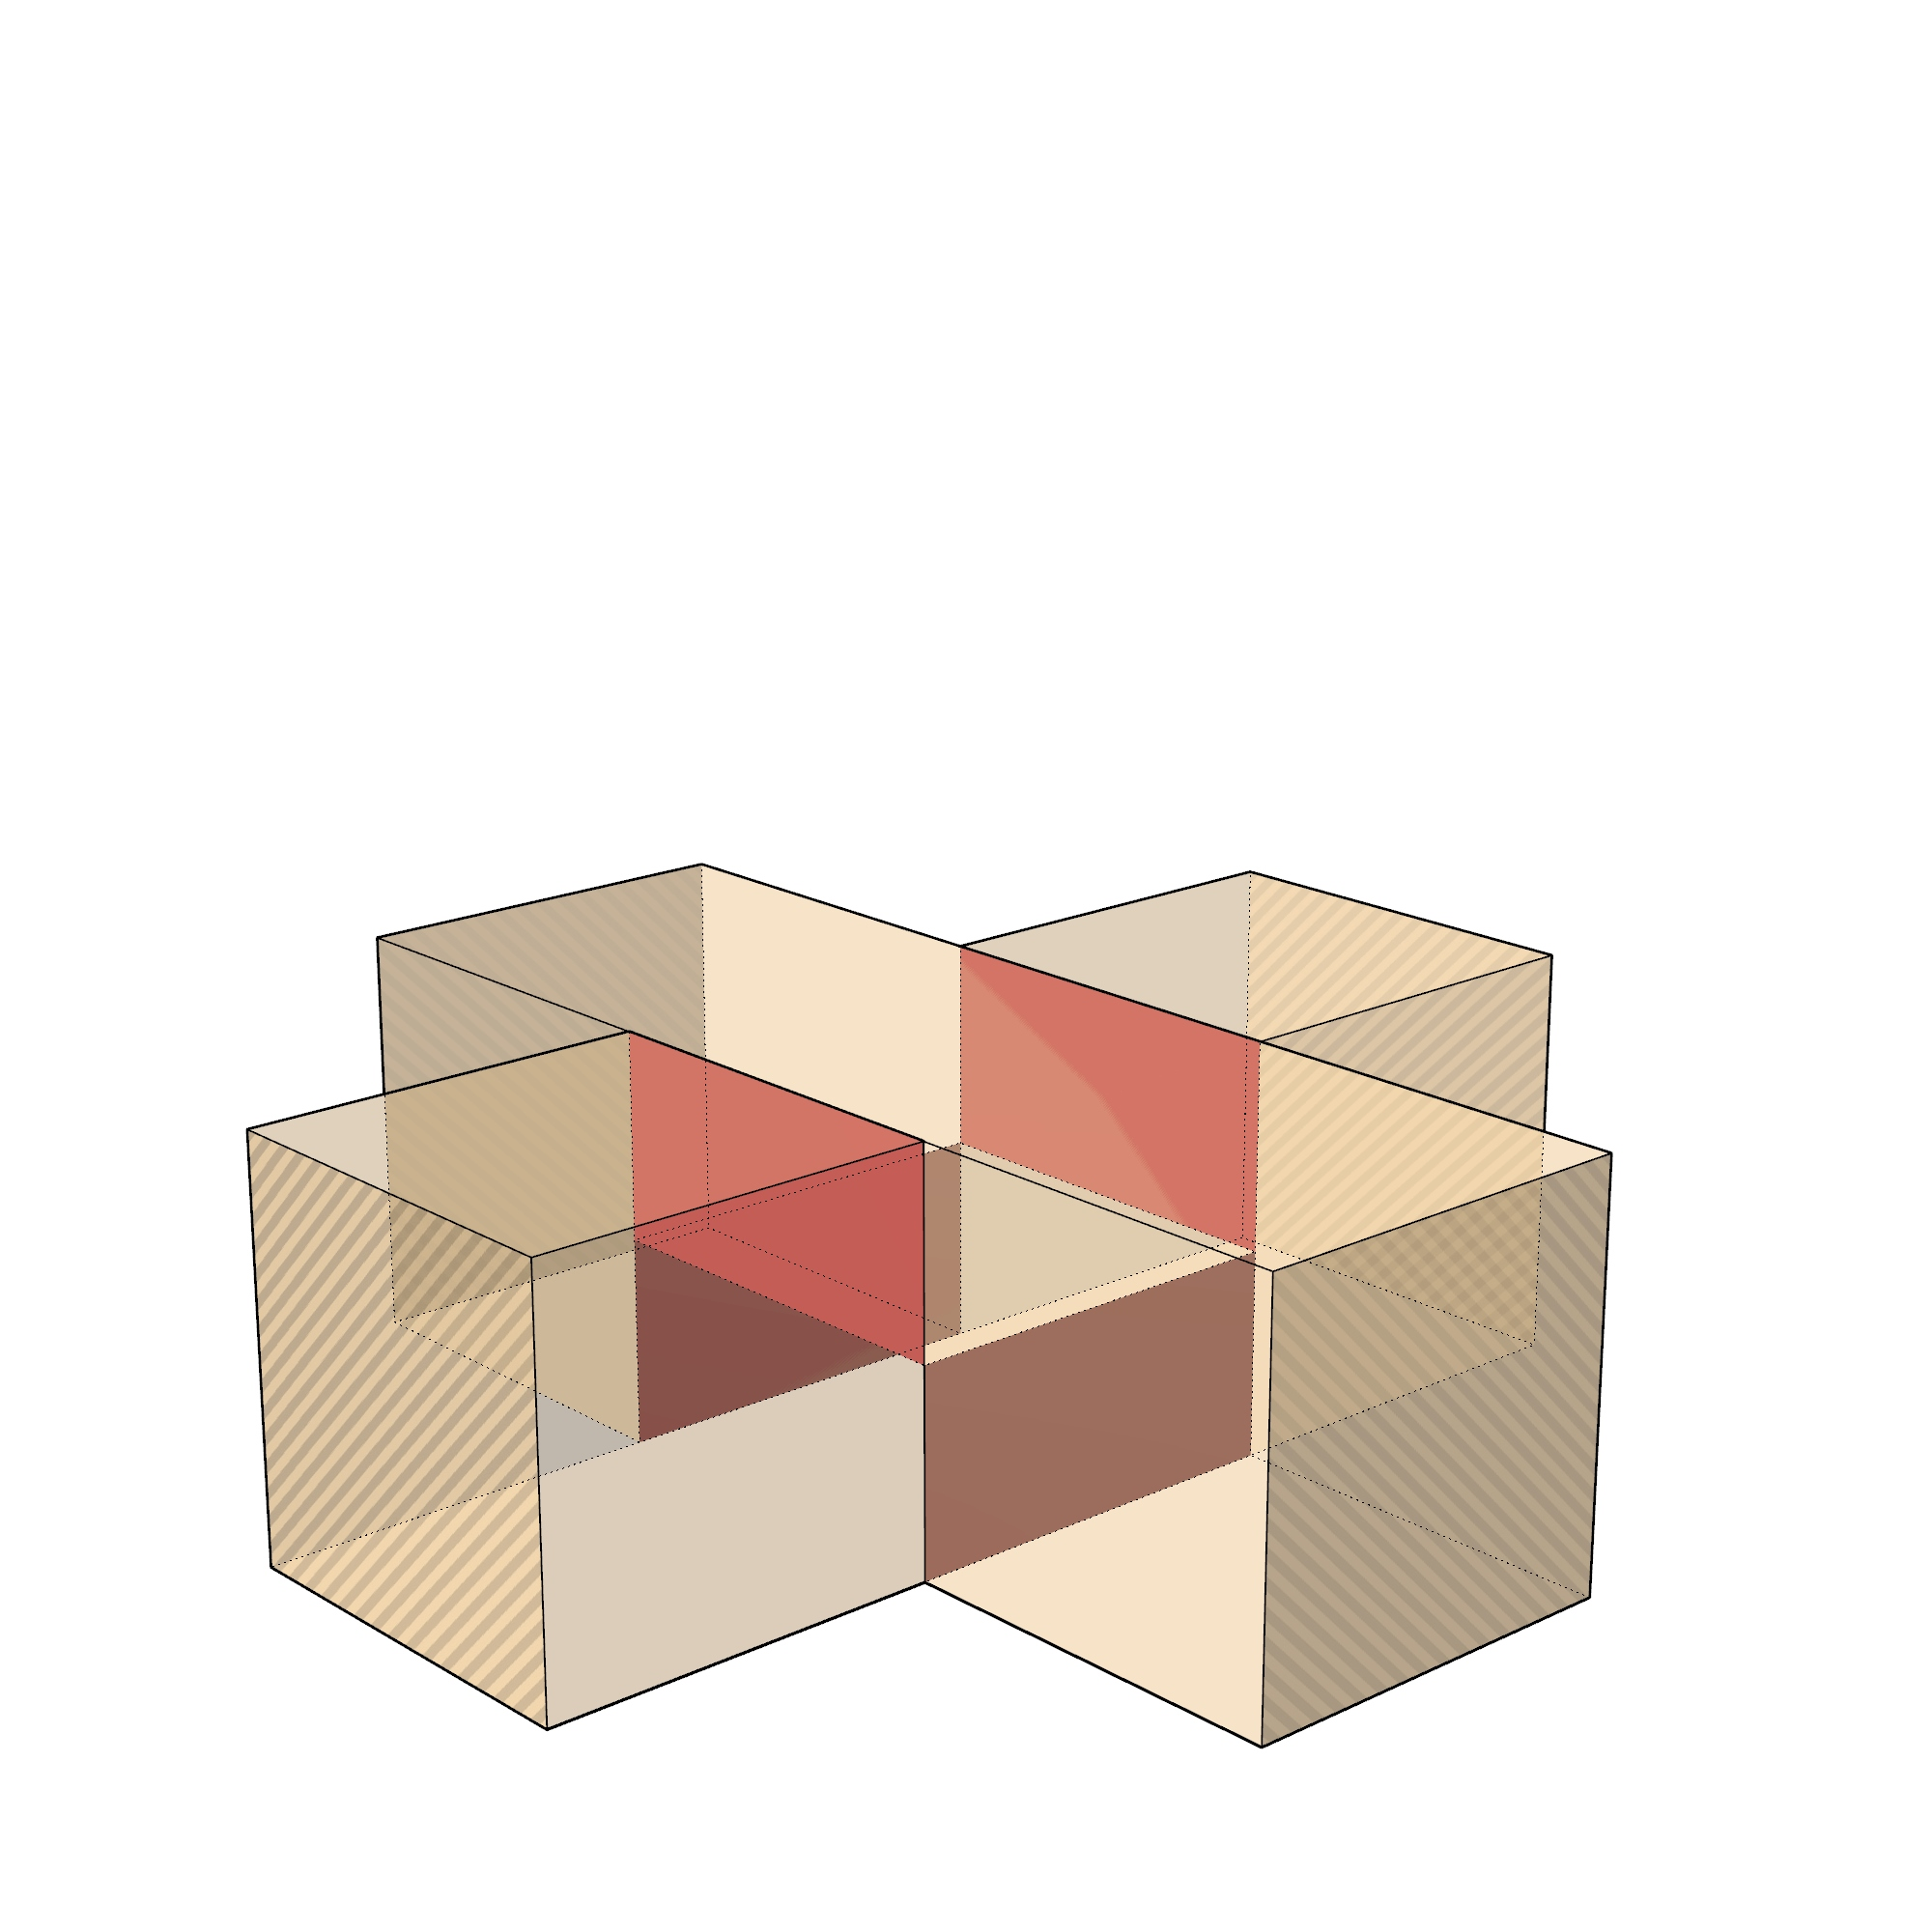
\includegraphics[width=\textwidth]{images/02/LapJoint_6.jpg}
         % \caption{SubFigureCaption}
         %\label{fig:uniquesubfigurelabel}
     \end{subfigure}
        \caption{Diagram of rubbing surfaces in a pair of half lap joints during assembly}
        \label{fig:rubbing-surface-in-lap-during-assembly}
\end{figure}

The design of these contact surfaces are used for many different purposes. For example to introduce geometrical interlock \parencite{larssonTsugiteInteractiveDesign2020, songRecursiveInterlockingPuzzles2012}, improve load transfer \parencite{likosEffectTenonGeometry2012}, improve structural stiffness \parencite{fangJoineryConnectionsTimber2018} or to improve stability against live load \parencite{jacksobonHistoricAmericanTimber2014}. Depending on the geometry of the sliding surface (e.g. tapered vs parallel) and the quality of the machined surface (e.g. rough vs smooth surface) these rubbing surfaces introduce different amounts of sliding friction that must be overcome by force.

Carpenters have always been aware of the quality of the joints and how it affects the assembly difficulty. However, with the use of CNC controlled joinery machines, the fabrication tolerance can be controlled much more easily. It is worth mentioning that one precedent project has attempted to control the moisture of the wood to shrink it for reducing friction \parencite{jennyPedagogyDigitalMateriality2022}. However the approach required heating the entire piece of wood, and would be difficult for larger scale structures.

\subsection{Tight Fitting Joints}
\label{subsection:challenges-tight-fitting-joints}

The second form of assembly-resistance is the fit of the mating joints. Fit is a measurement of the tightness of the connection between two mating parts. The fit can be categorised into three main types: clearance fit, transition fit, and interference fit. Clearance fit allows for some play between the parts, whereas interference fit requires force to assemble the parts and creates a tight, secure connection. Transition fit lies between these two extremes, providing a snug fit with some allowance for slight variations in the parts' dimensions.

Various factors can influence the fit of the mating joints, such as machining tolerances \parencite{thibautWoodMachiningFocus2016}, movement of the timber after machining due to release of stress, and environmental conditions such as temperature and humidity change \parencite{cochranTimberFrameLayout2018}. 

Tighter fits can result in higher frictional forces, which may require more force to overcome during assembly. It can also increase the difficulty for the robot to align the joints to begin assembly, which may increase the failure rate. Conversely, looser fits can lead to lower frictional forces but may compromise the structural integrity or performance of the assembled components \parencite{robellerRoboticIntegralAttachment2017}.

Existing studies on the effects of timber joint fit are mostly focused on furniture scale joinery using hardwood and with glue. \parencite{elekEvaluationEffectOptimal2020, koerner-al-rawiRoboticTimberAssembly2020, larssonTsugiteInteractiveDesign2020, likosEffectTenonGeometry2012} At the scale of timber frame construction, the choice of fit is typically based on the carpenter's experiences and historically proven norms \parencite{chappellTimberFramerWorkshop2011}. Only one recent study reported on the force required for architectural scale timber joints for plate structures \parencite{robellerRoboticIntegralAttachment2017}. 

In fact, much of the architectural scale robotic assembly research avoided the problem of tight fitting joinery at all due to the difficulty in assembling them, instead they use tangential connections \parencite{apolinarskaSequentialRoof2016, gandiaAutomaticPathPlanning2018, paraschoCooperativeRoboticAssembly2019}, and butt joints \parencite{apolinarskaRoboticAssemblyTimber2021, thomaRoboticFabricationBespoke2018} that did not require a large assembly force. However, these joint designs require an extra fastening step, such as glueing \parencite{gramaziokohlerresearchethzurichSemiramis2022, helmreichRoboticAssemblyModular2022} and screwing \parencite{apolinarskaSequentialRoof2016, thomaRoboticFabricationBespoke2018} that is often performed manually. Even when integral timber joinery was involved, a loose fit was chosen to make the robotic assembly process easier. 

\subsection{Assembly Force vs Robots}
\label{subsection:challenges-assembly-force-vs-robots}

The need to apply a large assembly force to overcome sliding friction and tight fit is a challenging problem for robotic assembly. 

Industrial robots, with their long kinematic chains are good for agile motions and spatial manipulation but are not optimal for applying large assembly force, typical industrial robots have payload capacity under 300kg, which roughly translates to 3kN of force. This is no match even against a reasonably tight timber joint at architectural scale. Even for special robots (e.g. palletizing and foundry robots) where the payload carrying capacity is high, they are bulky and heavy and are difficult to be integrated with a larger gantry system for architectural scale operation. 

The second challenging reason is that the large assembly force has to be applied directly on the mating joints. Considering that the most reasonable way for a robotic arm to hold a piece of timber would be from the middle, near its centre of gravity, the holding position would unlikely be where the joints are. For example, if a beam has two mating joints on the two ends, the pushing forces from the robotic arm would have to transfer through the length of the beam, by bending it, before it reaches the joints. Considering the low stiffness of the material, even if the robotic arm is strong enough, the strong pushing force would result in substantial bending or even damaging the beam. 

The third challenging reason is that there are more than one mating joint to be closed when assembling a beam. It is well known that the assembly of all the joints must proceed synchronously, or else the beam would jam and get stuck \parencite{dupontJammingWedgingConstrained1994}. Therefore, even if a robot could push from the centre of the beam without damaging it, any slight imbalance in the joint resistance among mating joints would result in a large torque on the wrist of the robotic arm. If the robot used a stiff control, this would likely result in an overload. If the robot used a compliant control, the beam would start to rotate and quickly get stuck. 

The fourth challenging reason is that a strong pushing force requires an equally strong reaction force that can support the other side of the mating joint. Therefore, even if a super robotic arm would be possible and the timber beam is not jamming, it is impossible to guarantee that the supporting force can be transmitted from the ground through the Partially Assembled timber structure without damaging what has already been built. The only possible alternative is to engineer a special end-effector to provide both the pushing force and the support at the same time, similar to the configuration of a clamp or a parallel gripper.

The fifth challenging reason is that the location and amount of timber frame joints can vary substantially between different elements in a timber frame structure. In addition, the shape of the joints are also variable, depending on the intersecting angles between the beams. Therefore even if a clamping end-effector concept is used, it is difficult to design it to accommodate different joint locations and joint angles. A severe limitation in the design possibilities would likely defeat the purpose of using robots to assemble structures in the first place. Perhaps this end-effector method would be possible for special cases where the joints are always at a similar location. For example, certain space frames with a topologically repetitive arrangement \parencite{apolinarskaRoboticAssemblyTimber2021, willmannNewParadigmsAutomatic2016}. 

An alternative approach that was considered is to use more than one robotic arm, each holding a clamping end effector near the joints. However, it is challenging to scale up for more complex arrangements as the number of robots will have to increase with the number of simultaneously assembled joints. While this may be possible for a two-robot scenario, more robots will simply not fit in the limited space between them.

\subsection{Joint Alignment}
\label{subsection:challenges-joint-alignment}

During the assembly of timber structures, it is necessary to accurately align the mating joints between the robot-sode and the stationary-side.

On the robot-side, the joints are located on the beam that is being held by the robot. Because these beams are assembled in non-repetitive locations, teaching cannot be used \seeref{subsection:introduction-inaccuracy-for-non-repetitive-targets}. Therefore the end-effector that holds the beam is subjected to unmonitored deviation. If the timber elements are long, a small orientation error can cause a large positional deviation at the joints that are located far away from the robot wrist. Furthermore, long timber elements may also be slightly bent (permanent and static) or deflect (dynamic) due to its own weight, which further increases the deviation at the location where the joints mate.

On the stationary-side, the joints are spread across different elements in the partially constructed structure. Due to accumulated installation error, or deformation of the partially assembled timber structure, the location of the joints can deviate from where they are supposed to be. Moreover, the deviation at each of the joints may move towards different directions, making alignment and correction difficult.

Because the robot targets are all extracted from a CAD model, unless there are active sensors monitoring the location of the joints on both sides, the joint pairs are likely to be subjected to misalignments which cannot be detected or corrected. Even if the misalignment can be detected, if there are more than one joint to align, correction may still be impossible due to conflicting deviation direction. If misalignment is severe and the problem is undetected, the subsequent robotic motion can cause damage to the timber parts. 

Precedence research in robotic timber assembly have attempted to solve this problem by using chamfered edge to guide the joints into alignment \parencite{robellerRoboticIntegralAttachment2017}. An active sensing and correction approach have also been proposed \parencite{apolinarskaRoboticAssemblyTimber2021}. Machine learning techniques was applied to teach a robot equiped with 
force-torque sensors to peform real-time adaptation.

\subsection{Fastener Installation}
\label{subsection:challenges-fastener-installation}

While many of the traditional timber frame joints contain no fasteners, some of them do, and for a multitude of reasons. For example:
\begin{itemize}
    \item \textbf{Timber wedges} are used to pull the joints tighter during assembly and can improve its stiffness
    \item \textbf{Timber dowels or pegs} are used to prevent joint loosening due to live load
    \item \textbf{Metal dowels} are used in contemporary designs to transmit shear force with metal plate connectors
    \item \textbf{Metal screws} can be used to transmit tensile forces over a joint that would be hard to achieve using timber contact faces alone
\end{itemize}

The assembly of threaded fasteners is a common operation in the manufacturing industry \parencite{jiaSurveyAutomatedThreaded2019}. Many different types of specialised end-effectors, robotic screwdrivers and screw feeding systems are designed to accommodate different types of screws. In timber construction, the automated assembly lines for prefabricated light-timber frame walls often have integrated screwdrivers and nail guns. Automated nailing has also been demonstrated for large-scale architectural construction \parencite{apolinarskaComplexTimberStructures2018, apolinarskaSequentialRoof2016}. However, most of these systems have been used for assembling planar assemblies and there are extra challenges when this has to be performed spatially. For example, handling long screws and non-orthogonal entry angles. Many of these precedence projects have resorted to assembling the screws manually \parencite{apolinarskaRoboticAssemblyTimber2021, thomaRoboticFabricationBespoke2018, willmannNewParadigmsAutomatic2016}. 

For timber frame construction with larger timber sizes, the screws used on the integral timber joints are often much larger than those used in the lighter timber systems. For other fasteners such as dowels and wedges, they are more specialised and have no automated precedence. 

\section{Computational and Design Challenges}
\label{section:challenges-computational-and-design-challenges}

\subsection{Designing with Integral Timber Joints}
\label{subsection:challenges-designing-with-integral-timber-joints}

Timber frame structures often employ the use of integral timber joints that are interlocking, to restrict the movement of beams after assembly. In many cases, there is only one single direction in which the mating beams can be moved to assemble the joints. The arrangement of beams and the design of the interlocking joints works together to provide the stability and stiffness of a timber frame structure. However, this approach also creates a complex, interlocking system of parts that are difficult to design and analyse, not unlike the 3D interlocking puzzles commonly found in museum gift shops.

Carpenters have long understood that a successful timber structure is not only one that stands up, but also one that can be assembled. In the pre-digital era, the scale and complexity of large timber structures, such as pagodas, roofs, and bridges, required the most experienced master carpenters to design \parencite{haymanTimberframedBuildings2021, hewettEnglishHistoricCarpentry2022, mullerHistoryDevelopmentStages2022, vandenabeeleJoiningTechniquesNineteenth2018}. Even today, one of the most challenging tasks when designing a complex timber structure is to ensure that the beams and their joints satisfy both structural and assembly requirements \parencite{chiltonTimberGridshellsArchitecture2016}.

\begin{itemize}
	\item Structural requirements include arranging beams into a stable and functional structural system and designing the joints to transmit structural forces. 

	\item Assembly requirements include ensuring that all components can be manoeuvred into place, accounting for the constraints imposed by the interlocking joints, and verifying that the assembly sequence does not create conflicts or blockages \parencite{wangStateArtComputational2021}. 

\end{itemize}
Historically, successful timber frame designs were passed from one generation of carpenters to the next, each of them making iterative improvements. Particularly successful designs, such as post-and-beam structures and long-span roof trusses became a typology that was repeated and used many times \parencite{sobonTimberFrameConstruction1984, jacksobonHistoricAmericanTimber2014}.

Today, advances in the computer graphic field have created many analytical methods and opened up new possibilities for designing and analysing novel timber structures. In this thesis, structural analysis and assembly analysis will not be the core focus of the research. This is because they are already a highly established field and that many existing works have already studied them in depth. However, it is still necessary to be aware of their challenges to be able to apply the techniques correctly.

\subsection{Structural Analysis}
\label{subsection:challenges-structural-analysis}

Timber structures are designed by considering various factors such as material properties, structural loads, environmental conditions, building codes, and aesthetics. The process typically begins with architectural design, where the overall form and layout of the building are determined. This is followed by structural design, where the appropriate sizes and shapes of timber members, connections, and joints are selected to ensure structural integrity, stability, and longevity.

Timber structures, particularly those with integral timber joints, present unique challenges in terms of analysis due to the complexity of the joint behaviour, material properties, and load distribution. These challenges can make it difficult to accurately predict the structural performance and ensure the safety and longevity of the structure. Some of the key challenges in analysing integral timber joints are:

\begin{itemize}
	\item \textbf{Anisotropic material properties --} The mechanical properties of wood material vary along different directions. This anisotropy can affect the behaviour of integral joints, as the strength and stiffness of the joint depend on the direction of the applied loads and the orientation of the wood fibres. Accurate analysis must account for these variations in material properties \parencite{thelanderssonTimberEngineering2003}.

	\item \textbf{Non-linear behaviour --} The behaviour of timber material and timber joints can be non-linear, particularly under high load levels or in the presence of defects, such as cracks or knots. This non-linear behaviour can complicate the analysis process, as it requires more advanced numerical methods and computational models to accurately predict joint performance \parencite{gustafssonFracturePerpendicularGrain2003, tanadiniAnalysisDesignTimbertotimber2021}.

	\item \textbf{Moisture content and hygroscopicity --} Wood is hygroscopic, meaning it absorbs and releases moisture in response to changes in environmental conditions. This can cause dimensional changes and affect the mechanical properties of the timber, impacting the behaviour of integral joints. Accurate analysis must account for these moisture-related effects and their potential impact on joint performance \parencite{thelanderssonTimberEngineering2003}.

	\item \textbf{Load distribution and interaction --} Integral timber joints often involve complex load distribution and interaction between multiple components. This can make it difficult to accurately predict the load-carrying capacity and failure modes of the joint. Advanced structural analysis techniques, such as Finite Element Analysis (FEA), are often required to accurately model these interactions and predict joint behaviour.

	\item \textbf{Uncertainty in material properties and geometric tolerances --} Variability in material properties, such as strength and stiffness, as well as uncertainties in geometric tolerances, can make it challenging to predict the behaviour of integral timber joints with high confidence. Probabilistic approaches, such as reliability analysis \parencite{ranta-maunusReliabilityAnalysisTimber2001} and stochastic finite element methods \parencite{kandlerStochasticFiniteElement2015} can be used to quantify these uncertainties and assess the impact on joint performance.

\end{itemize}
\subsection{Assembly Analysis}
\label{subsection:challenges-assembly-analysis}

Assembly analysis of timber frame structures with integral timber joints is a crucial aspect to ensuring the structure can be assembled, this is known as joint mobility analysis, or assemblability analysis. The assembly analysis can be extended to include automatic sequence planning and motion planning \parencite{wangStateArtComputational2021}. Assembly problems can be further categorised \parencite{wangStateArtComputational2021} by their properties: 

\begin{itemize}
	\item \textbf{Number of hands --} number of simultaneously moving parts needed for assembly 

	\item \textbf{Monotonicity --} whether the parts can be assembled in one simple motion, or whether intermediate movements are needed.

	\item \textbf{Linearity --} whether the assembly motions are linear, rotational, helical or other freeform motions. 

\end{itemize}
Most of the precedence robotic assembly projects in the architectural field, including the timber frame assembly problem in this thesis, belong to the simplest option of all (single hand, linear and monotonic movements). Even for projects that have used more than one robot during the process \parencite{paraschoCooperativeRoboticAssembly2019, thomaRoboticFabricationBespoke2018}, unless it involves multiple simultaneous movements in different trajectories, they are still considered one-hand problems.


Large amount of research has been devoted to the automatic sequence and motion planning. For example, in the context of mechanical assembly \parencite{bahubalendruniReviewAssemblySequence2016, defazioSimplifiedGenerationAll1987, homemdemelloTaskSequencePlanning1989, wilsonGeometricAssemblyPlanning1992b}, computer graphics \parencite{natarajanPlanningAssemblies1988, wangDESIAGeneralFramework2018} and also timber construction \parencite{taiDesignAssemblyComputational2012}. It is also possible to include additional heuristics in the search of an optimal assembly plan. For example, to maximise structural stability during construction \parencite{deussAssemblingSelfsupportingStructures2014, garrettScalableProbabilisticallyComplete2020}, avoid robotic collision \parencite{huangFrameFabRoboticFabrication2016, yuHighlyInformedRobotic2016} or to minimise assembly time.

When robots are used to perform an assembly task, the assembly analysis mentioned above also has to consider the actions of the robots and the tools, and their physical limitations. These limitations include:

\begin{itemize}
    \item \textbf{Collision --} The robot and parts attached to the robot must not come into collision among itself or with stationary objects \seeref{subsubsection:exploration-2-collision-checking}.

	\item \textbf{Reachability --} The robot must be able to reach all the targets that are needed to manipulate the objects for their assembly \seeref{subsubsection:exploration-2-inverse-kinematics}.

	\item \textbf{Payload and Accuracy --} Certain operations may not be possible due to the mechanical limitations of the robot.
\end{itemize}

The extension of these analysis into the design process includes:

\begin{itemize}
	\item \textbf{Automatic Sequence Planning --} Identical to the sequence planning above, concerned with the sequence among parts.

	\item \textbf{Automatic Task Planning --} Planning the discrete actions of the robot to assemble each part \parencite{homemdemelloTaskSequencePlanning1989}. For example, open gripper, move robot, and close gripper. 

	\item \textbf{Automatic Motion Planning --} Finding the trajectory for the robot joint to follow, such that the attached end-effector moves from one target to another \parencite{lavallePlanningAlgorithms2006}. 
\end{itemize}

In this thesis, task planning and motion planning are unavoidable for generating the robot programmes. However, sequence planning will not be studied. It is assumed that an experienced timber engineer, designer or carpenter can be tasked to determine the assembly order based on experience and intuition.

\subsection{Task and Motion planning}
\label{subsection:challenges-task-motion-planning}

The use of robots for assembling timber structures requires careful planning and simulation to ensure that there are no unintended collisions. 

The basic task of picking up a beam carrying it to the assembly location may sound simple for a human worker. However, the planning work required for a robot to do the same is not only computationally hard, but also complicated to set up correctly. The parameters that have to be planned are:

\begin{itemize}
	\item \textbf{Tasks --} What are the sequence of operations for moving the robot joints and actuating the attached tools (e.g. opening and closing grippers)?

	\item \textbf{Grasp --} What pose (position and orientation) does the robot use to hold the beam? Does the robot need to change its grasp during the process?

	\item \textbf{Targets --} Where are the targets for the robot to reach at the start and end of a motion to pick or place a workpiece at the correct location?

	\item \textbf{Trajectories --} What is the continuous path (a series of static joint angles) that allows the robot and its attached objects to move from one target to the next?

\end{itemize}
The main challenge for spatial assembly is that there are many possible directions and orientation for assembling an element. This is in steep contrast to a layer-by-layer construction approach, where new elements can be assembled from the top \parencite{apolinarskaSequentialRoof2016, gramaziokohlerresearchethzurichStackedPavilion2009}. 

Many spatial assembly projects have used a rule-based strategy to programme the transfer path. For example, a common approach for beam transfer is to raise the beam to a safe height before traversing horizontally \parencite{hackStructuralStayinplaceFormwork2020, sondergaardTopologyOptimizationRobotic2016}. However, this approach is still limited by the obstacles at the final approach when the robot is near the partially-assembled structure. For structures that are assembled from the core towards the periphery, a strategy of approaching the target from the ‘outside’ can be used \parencite{adelDesignRoboticallyFabricated2018}. 

A more generic strategy is to use a sampling-based motion planner as it has the ability to automatically search for a viable path while avoiding collisions \parencite{gandiaAutomaticPathPlanning2018, thomaRoboticFabricationBespoke2018}. This is critical if some of the beams have to reach into the small openings of a structure. However, one of the often cited knowledge gap remains at the automatic generation of robotic trajectories for large amounts of uniquely shaped and positioned elements \parencite{eversmannRoboticPrefabricationTimber2017, gandiaAutomaticPathPlanning2018}. Latest research developments have already created the interface to access planning tools from the robotics research field for planning architectural assemblies \parencite{gandiaAutomaticPathPlanning2018, paraschoCooperativeFabricationSpatial2017a, paraschoComputationalDesignRobotically2018}. The most comprehensive method to date being a unified sequence and motion planning or a unified task and 

\subsection{Joint Modeling and Solving}
\label{subsection:challenges-joint-modeling-solving}

Joint Modeling and Solving refers to the computational process of creating and adjusting parametric models of integral timber joints, ensuring their compatibility and adaptability within the larger context of the timber frame assembly, while taking into account fabrication constraints, user customizations, and structural considerations.

Timber joints are typically modelled as a subtraction from the beam’s geometry. In many joint designs, both halves of the joints are not geometrically similar, therefore the subtraction geometries for the beams on each sides are also different. In order to ensure correct fit, it is necessary to ensure that both sides of the joint will match with each other. While this is relatively straightforward to achieve for one joint instance, a parametric joint model will need to adapt itself to different jointing angles between the beams. Because of the continuous nature of the joining angles, the model requires defining parametric geometrical relationships in 3D to create the solid models \parencite{vestartasDesigntoFabricationWorkflowRawSawnTimber2021}. In general, a parametric joint model will contain fixed properties that are dependent on the neighbouring beams, and editable properties that can be customised:

\textbf{Adaptation to the intersecting beams' position, size and angle --} This adaptability allows the joint geometry to be computed automatically by the intersecting beams without explicit modelling. Thus, changing the intersecting beams’ locations can trigger an update to snap it to a new position. Figure \ref{fig:mortise_tenon_different_angles} shows a mortise and tenon joint adapting to different beam intersection angles.



\begin{figure}[htb]
     \centering
     \begin{subfigure}[b]{0.19\textwidth}
         \centering
         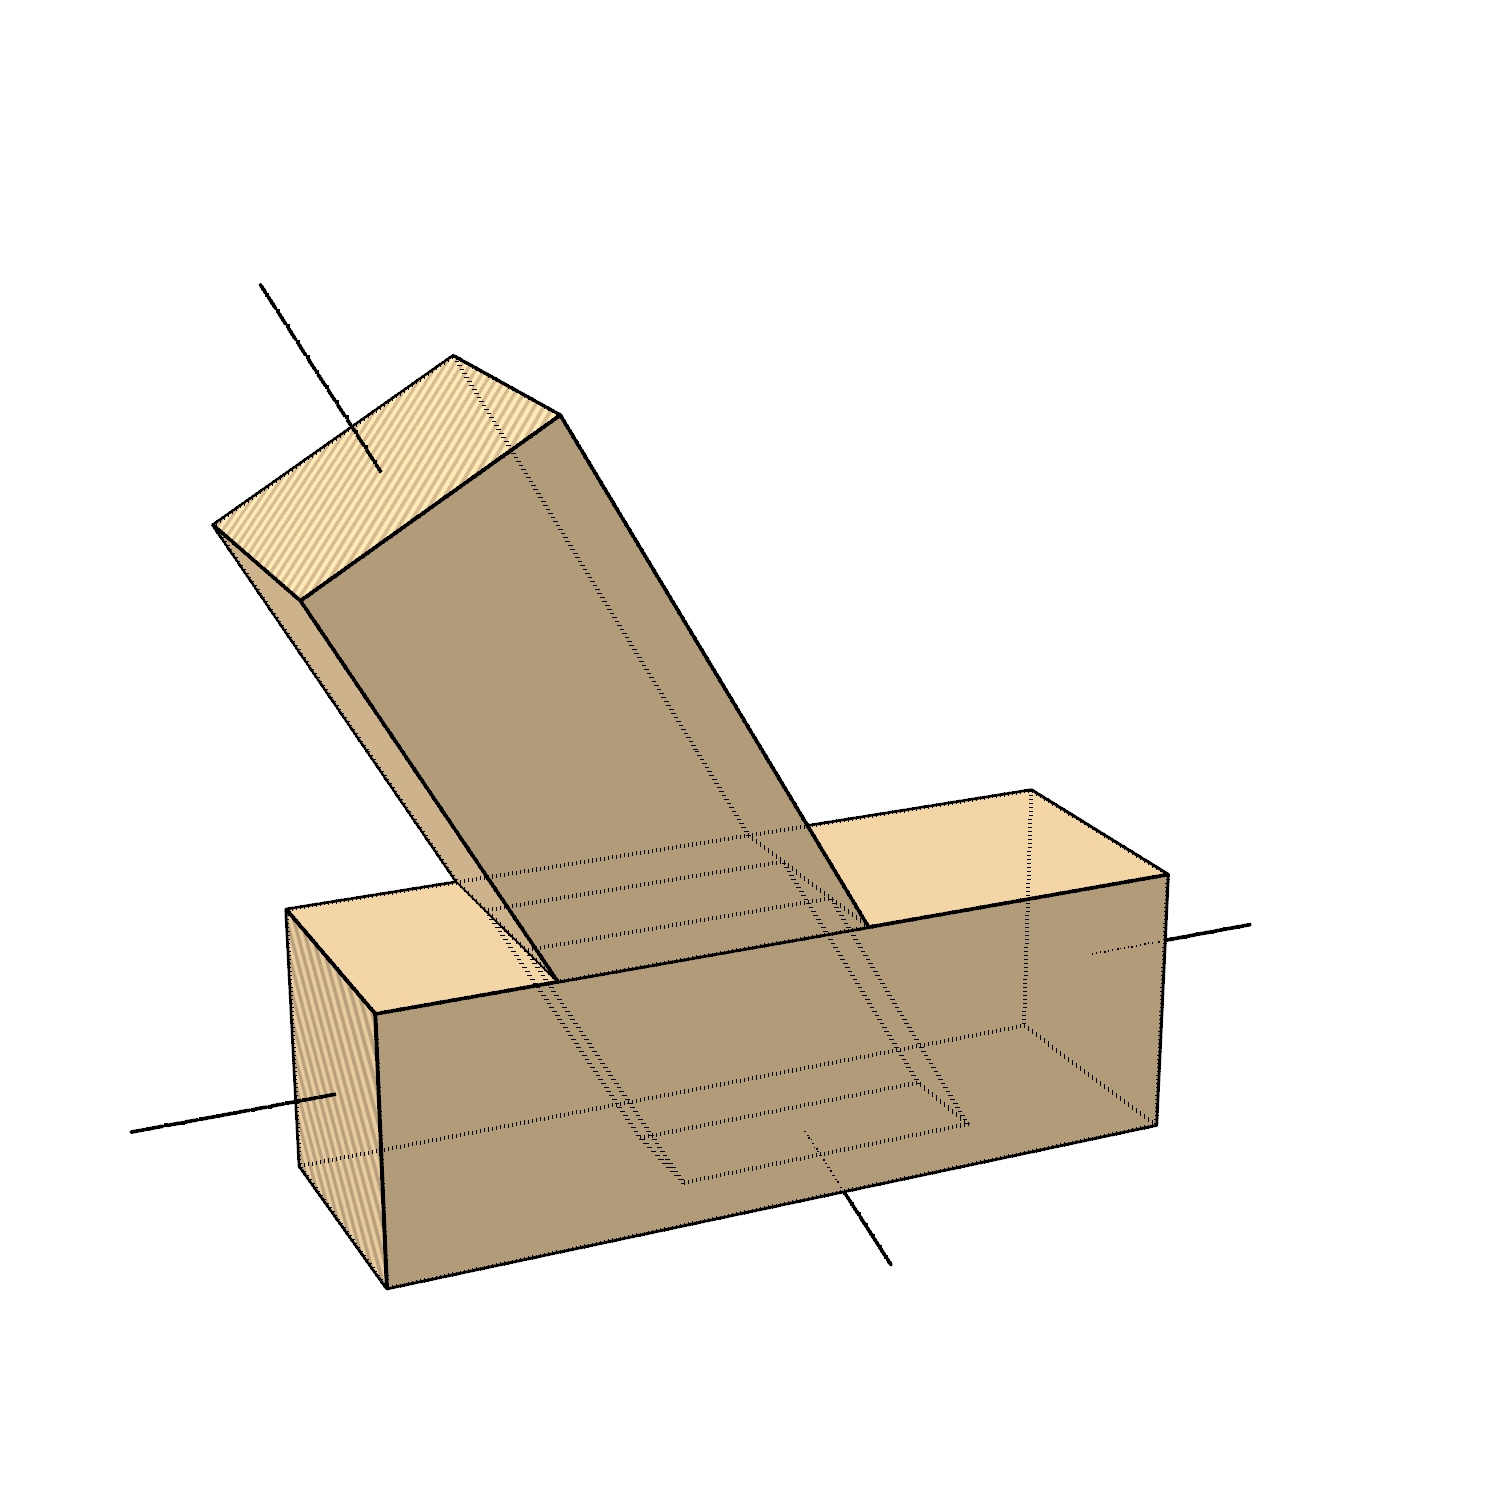
\includegraphics[width=\textwidth]{images/02/Tenon_3.jpg}
         % \caption{SubFigureCaption}
         %\label{fig:uniquesubfigurelabel}
     \end{subfigure}
     \hfill
     \begin{subfigure}[b]{0.19\textwidth}
         \centering
         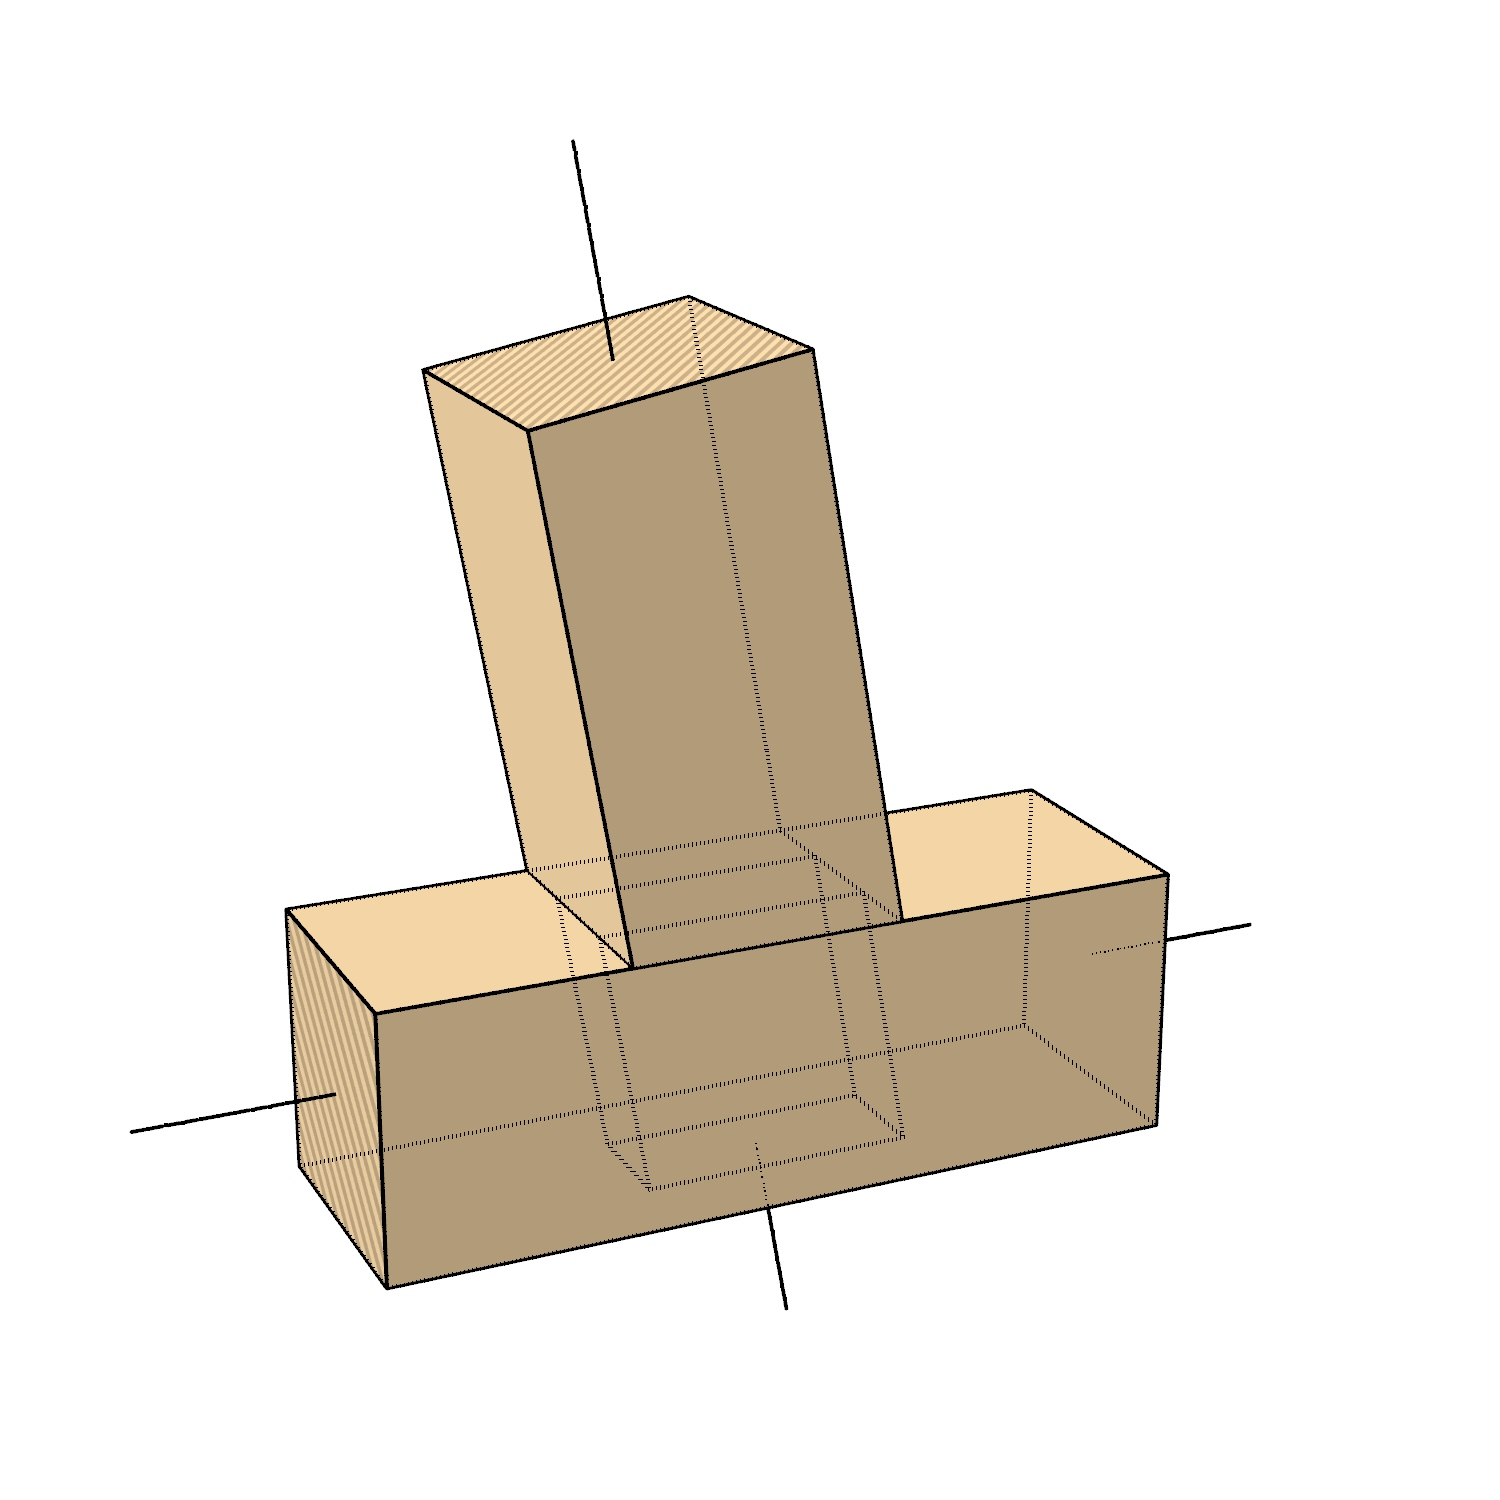
\includegraphics[width=\textwidth]{images/02/Tenon_1.jpg}
         % \caption{SubFigureCaption}
         %\label{fig:uniquesubfigurelabel}
     \end{subfigure}
     \hfill
     \begin{subfigure}[b]{0.19\textwidth}
         \centering
         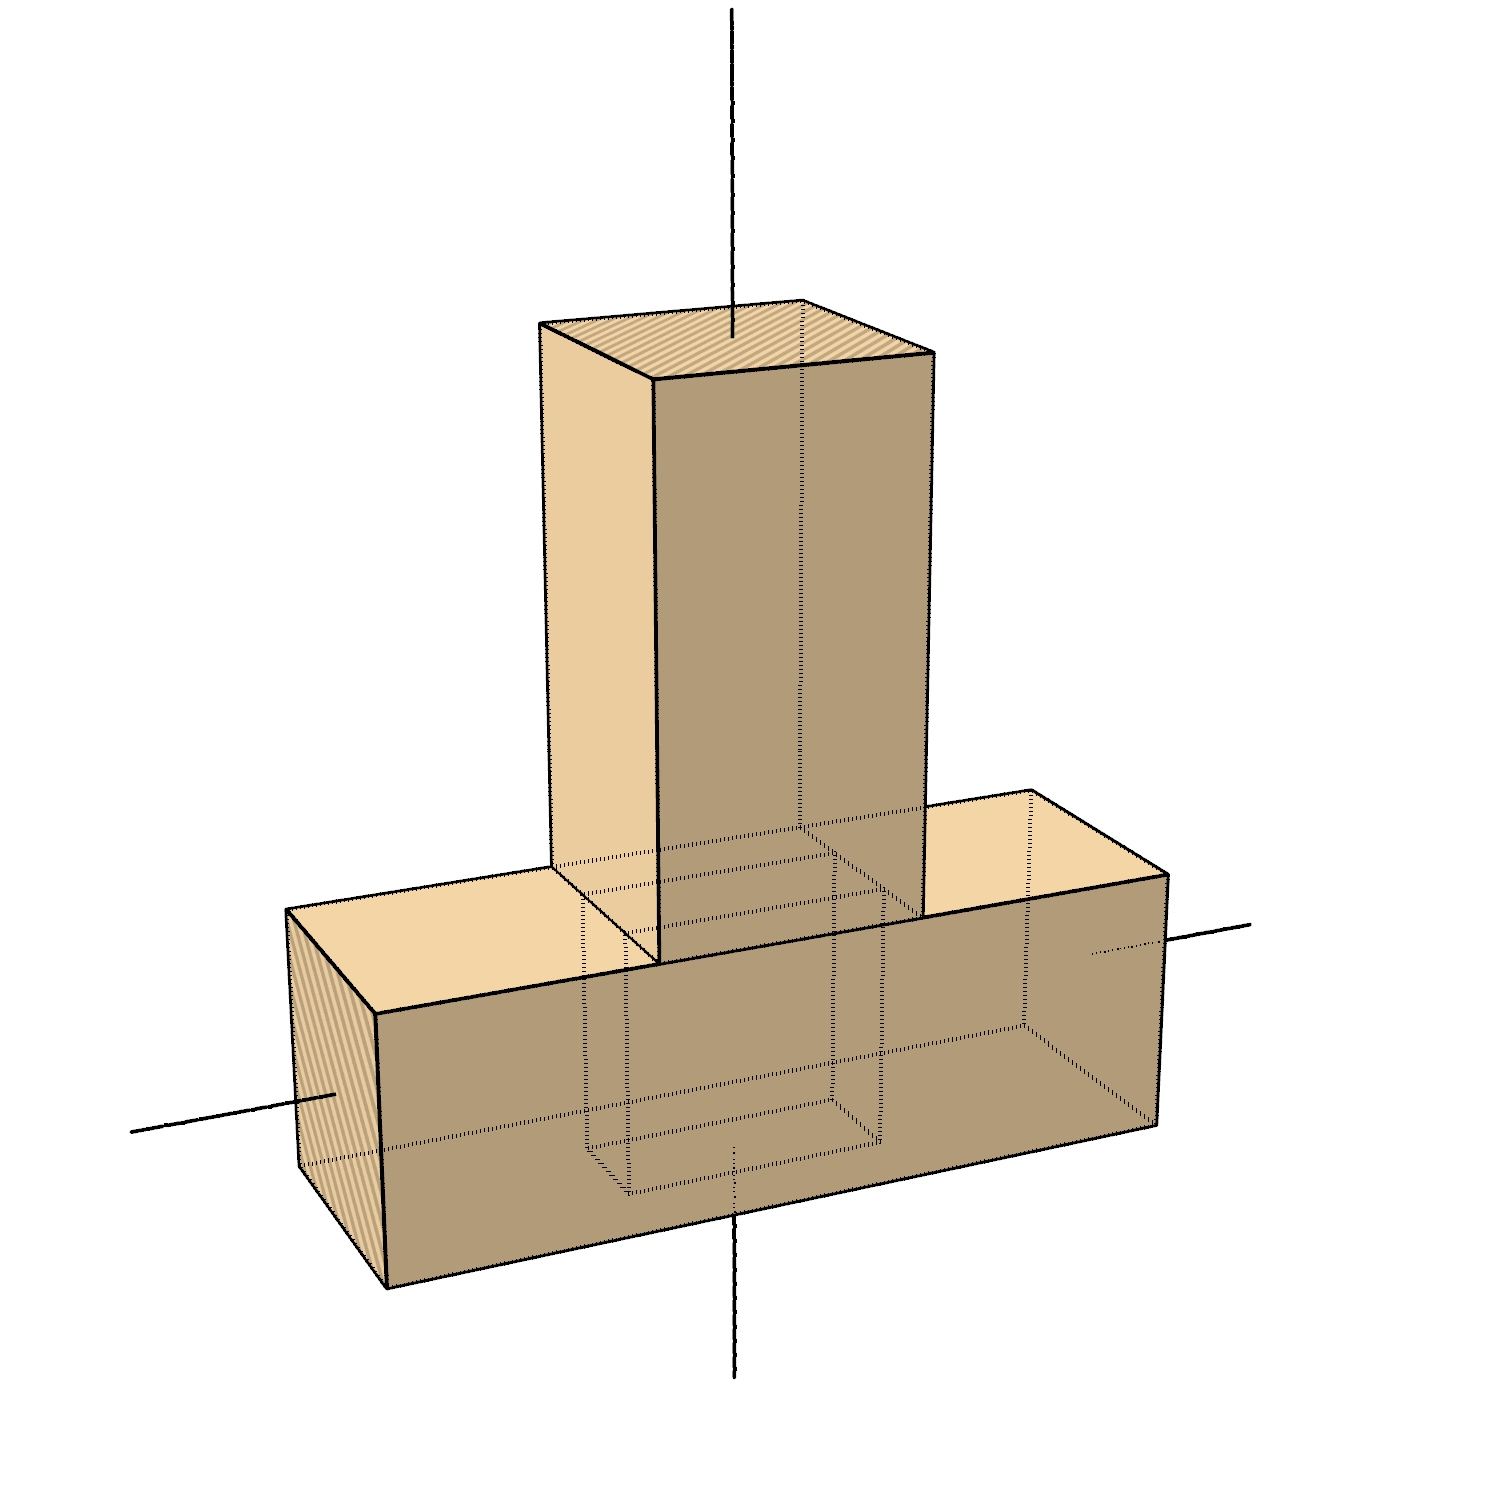
\includegraphics[width=\textwidth]{images/02/Tenon_0.jpg}
         % \caption{SubFigureCaption}
         %\label{fig:uniquesubfigurelabel}
     \end{subfigure}
     \hfill
     \begin{subfigure}[b]{0.19\textwidth}
         \centering
         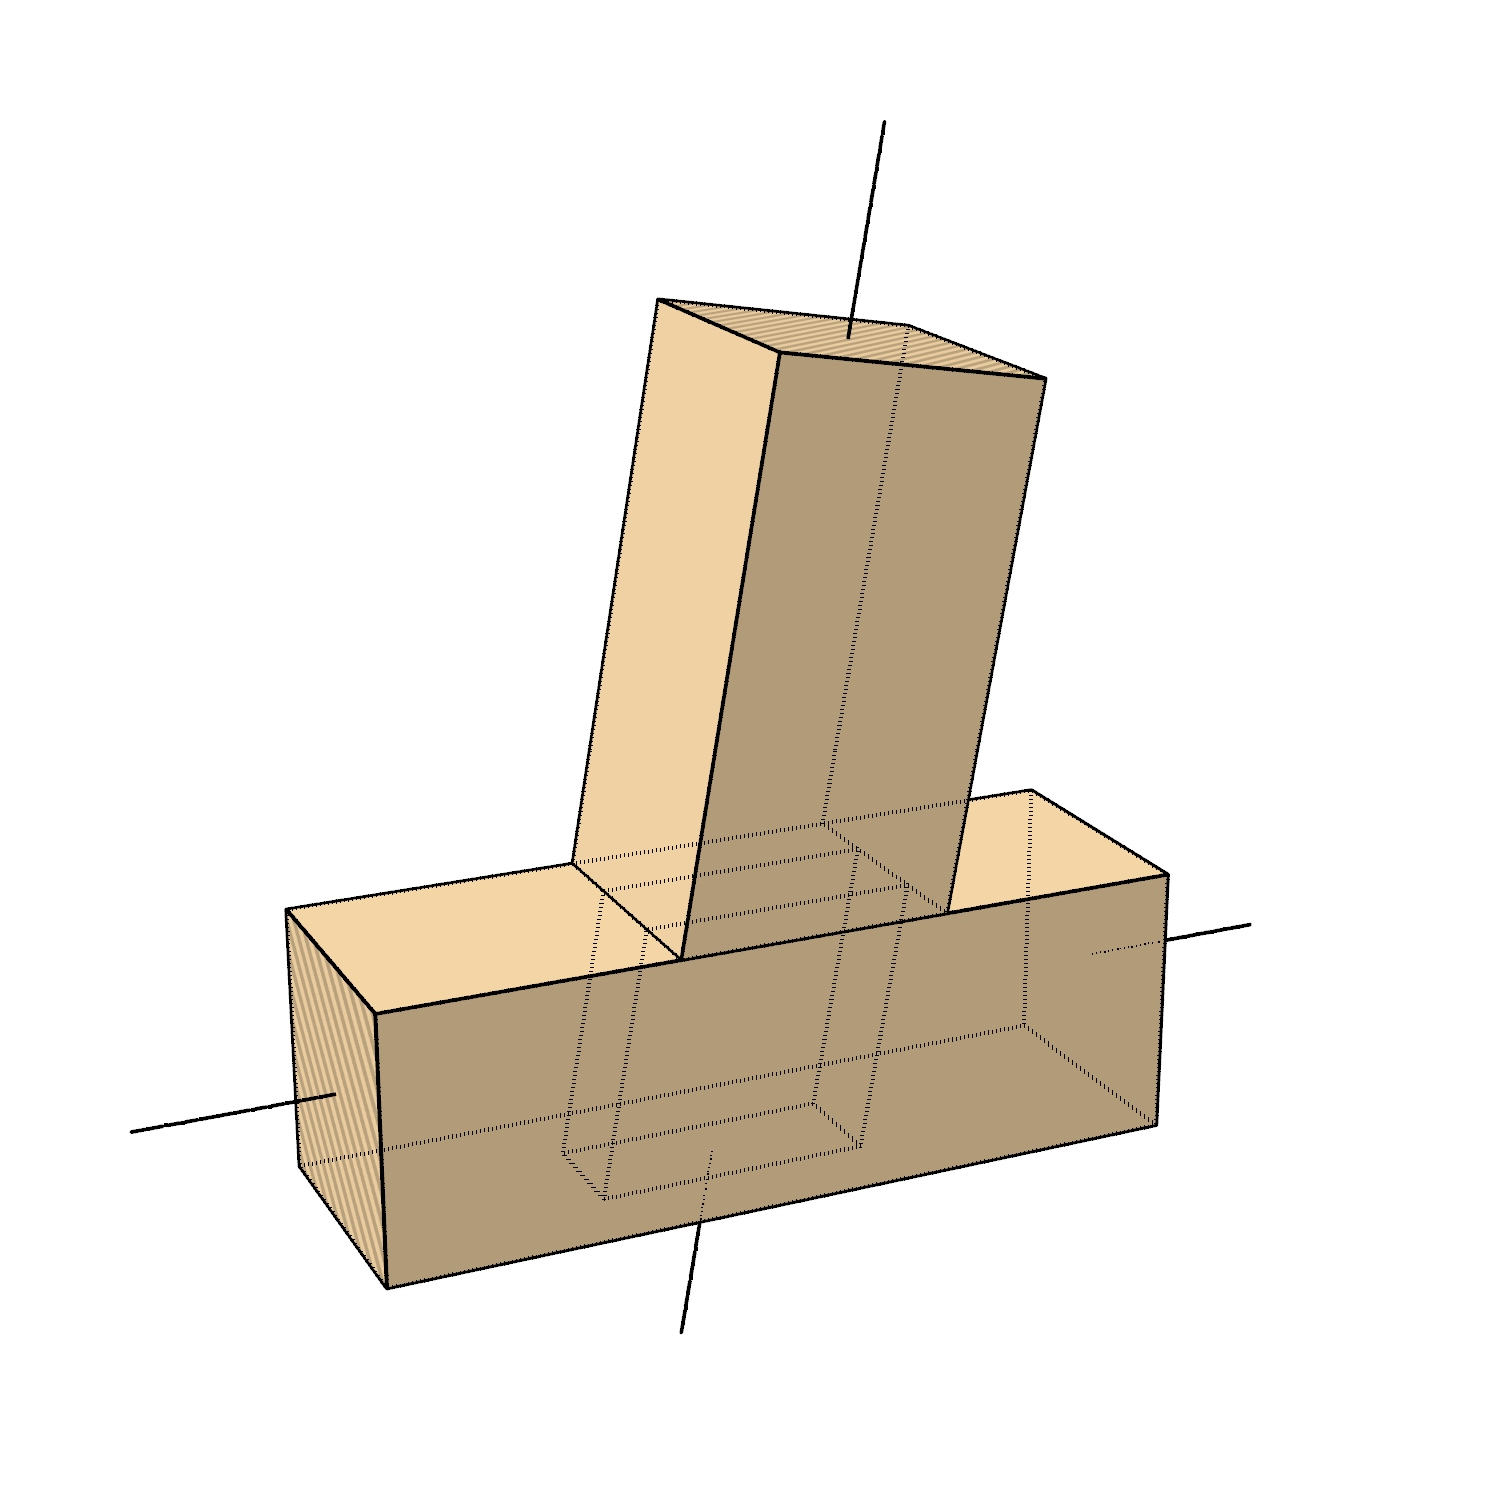
\includegraphics[width=\textwidth]{images/02/Tenon_4.jpg}
         % \caption{SubFigureCaption}
         %\label{fig:uniquesubfigurelabel}
     \end{subfigure}
     \hfill
     \begin{subfigure}[b]{0.19\textwidth}
         \centering
         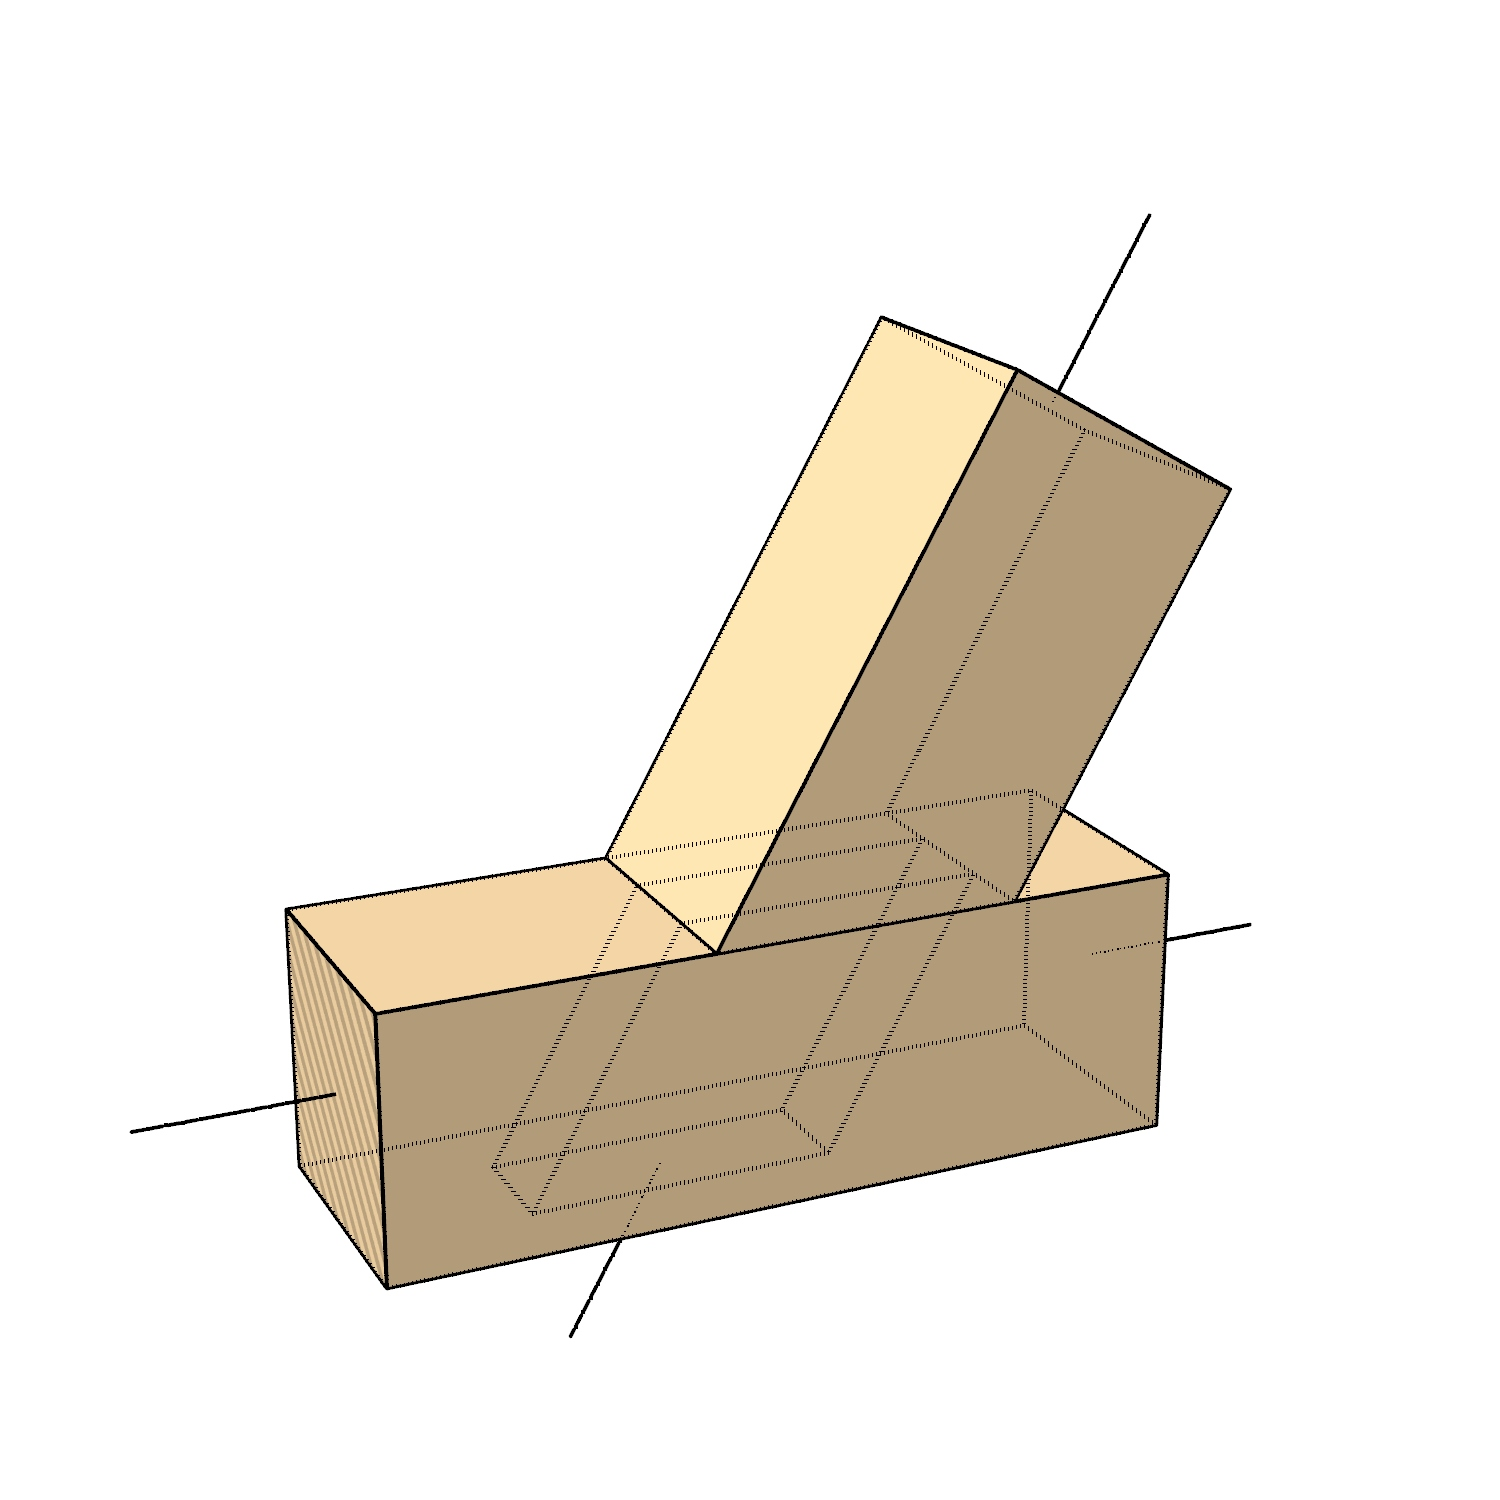
\includegraphics[width=\textwidth]{images/02/Tenon_6.jpg}
         % \caption{SubFigureCaption}
         %\label{fig:uniquesubfigurelabel}
     \end{subfigure}
        \caption{Example of a mortise and tenon joint adapting to different beam intersection angles}
        \label{fig:mortise_tenon_different_angles}
\end{figure}

\paragraph{Customization of detail sizes or proportions}
Even a simple lap joint model can include an adjustable parameter for the cheek depth. More complex joint topology can have many adjustable parameters \textit{(refer to the diagram of a housed dovetail T Lap having many parameters)}. These adjustments are often useful for changing the structural behaviour of the joint and may be specified or changed at a later stage of the design process during engineering calculations. Figure \ref{fig:mortise_tenon_different_topologies} show a mortise and tenon joint having the same intersection angles but different topologies. The proportion of the details in each topology would require a parametric definition.

\begin{figure}[htb]
     \centering
     \begin{subfigure}[b]{0.19\textwidth}
         \centering
         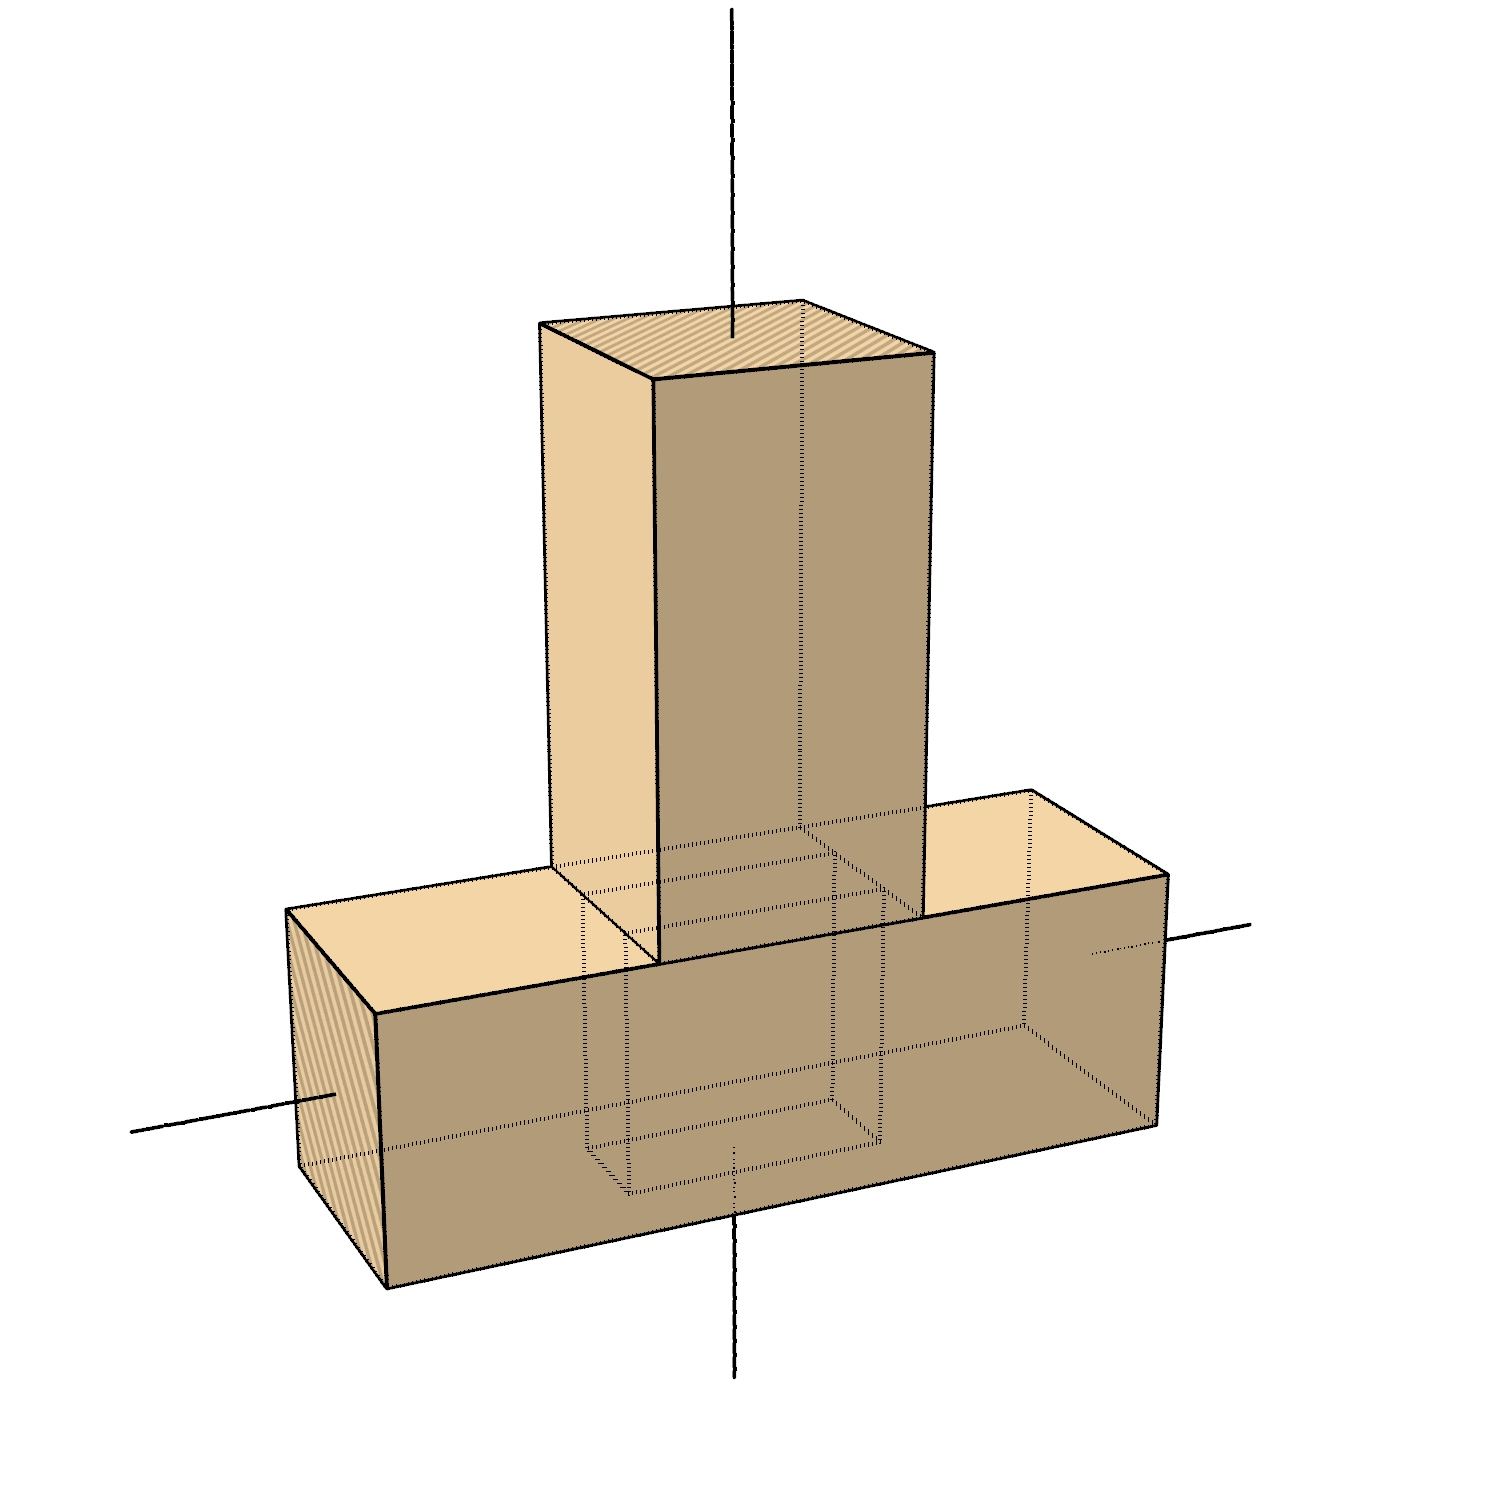
\includegraphics[width=\textwidth]{images/02/Tenon_0.jpg}
         % \caption{SubFigureCaption}
         %\label{fig:uniquesubfigurelabel}
     \end{subfigure}
     \hfill
     \begin{subfigure}[b]{0.19\textwidth}
         \centering
         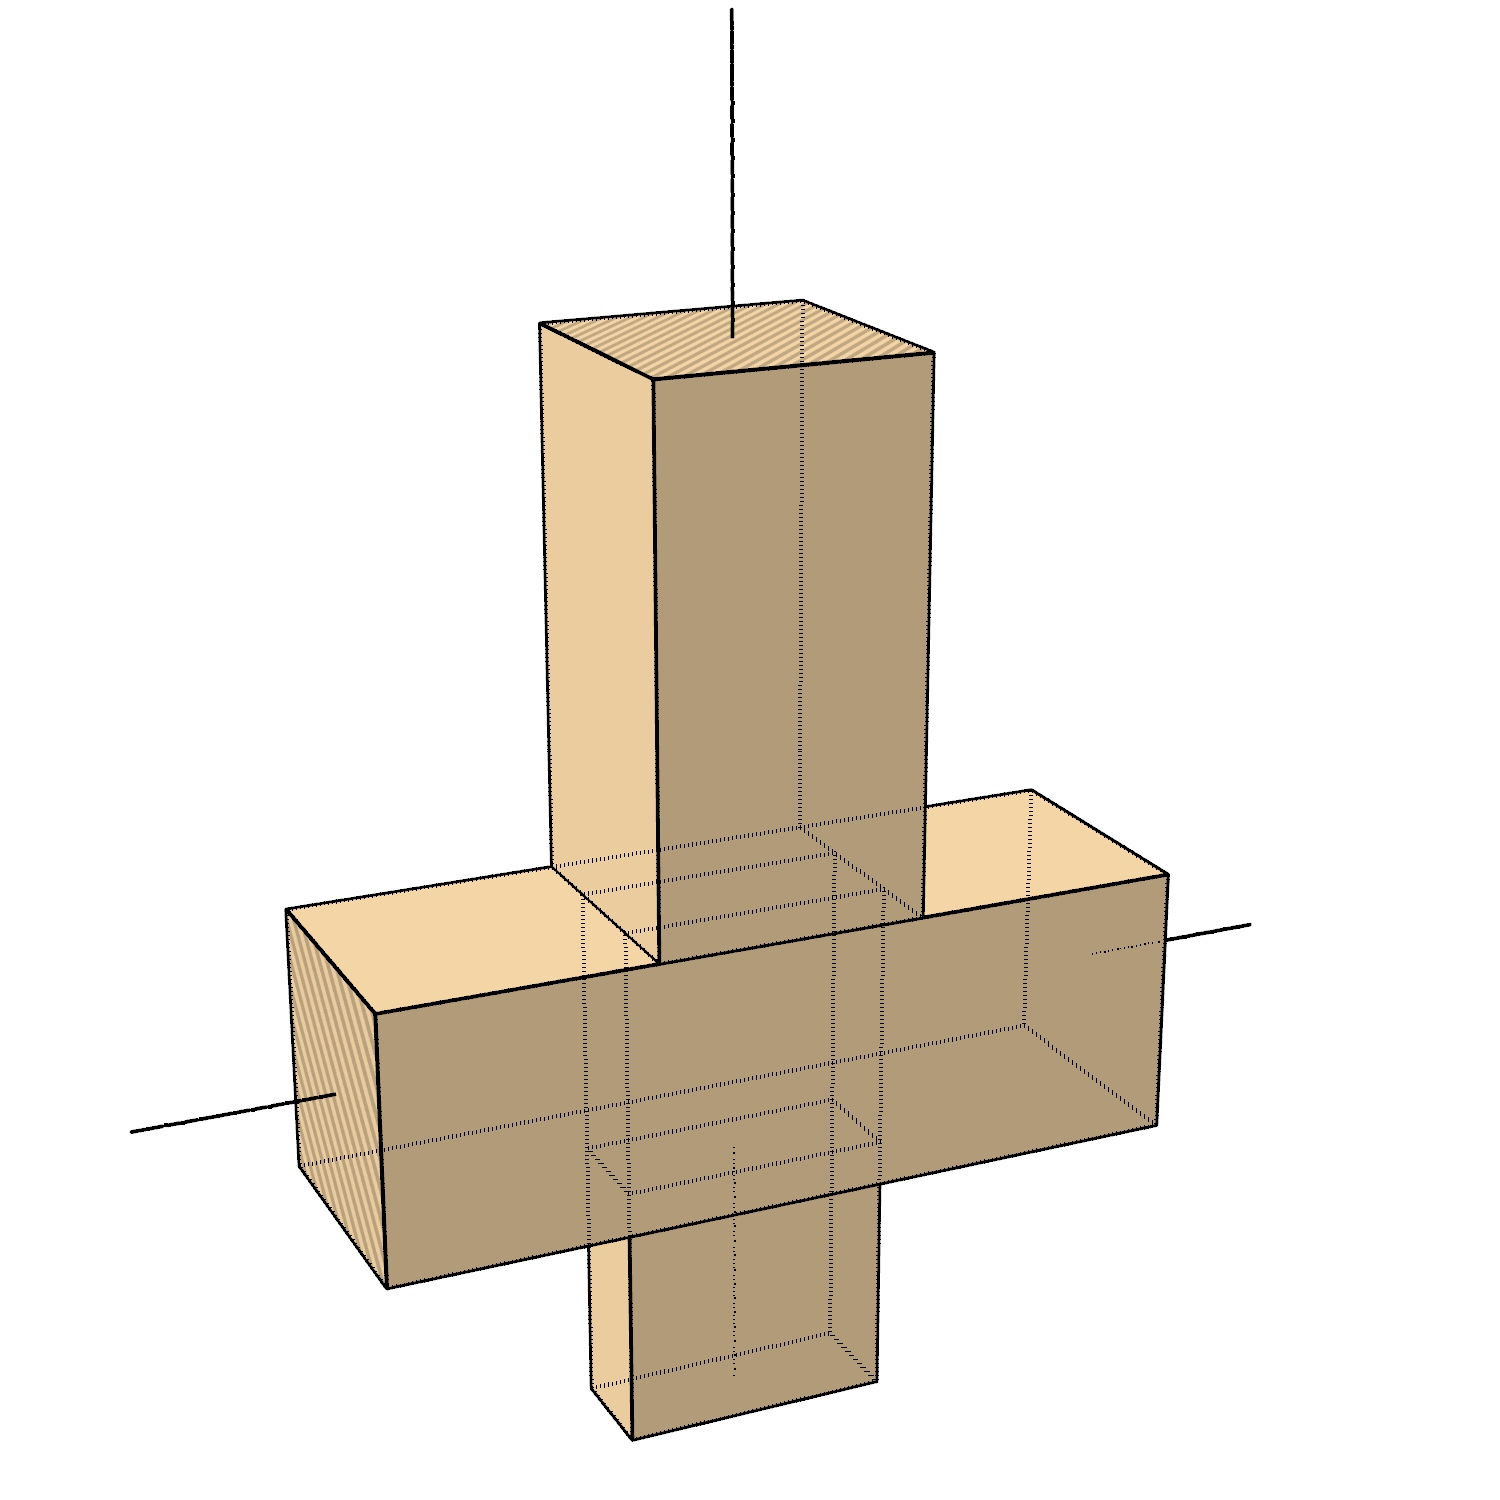
\includegraphics[width=\textwidth]{images/02/Tenon_9.jpg}
         % \caption{SubFigureCaption}
         %\label{fig:uniquesubfigurelabel}
     \end{subfigure}
     \hfill
     \begin{subfigure}[b]{0.19\textwidth}
         \centering
         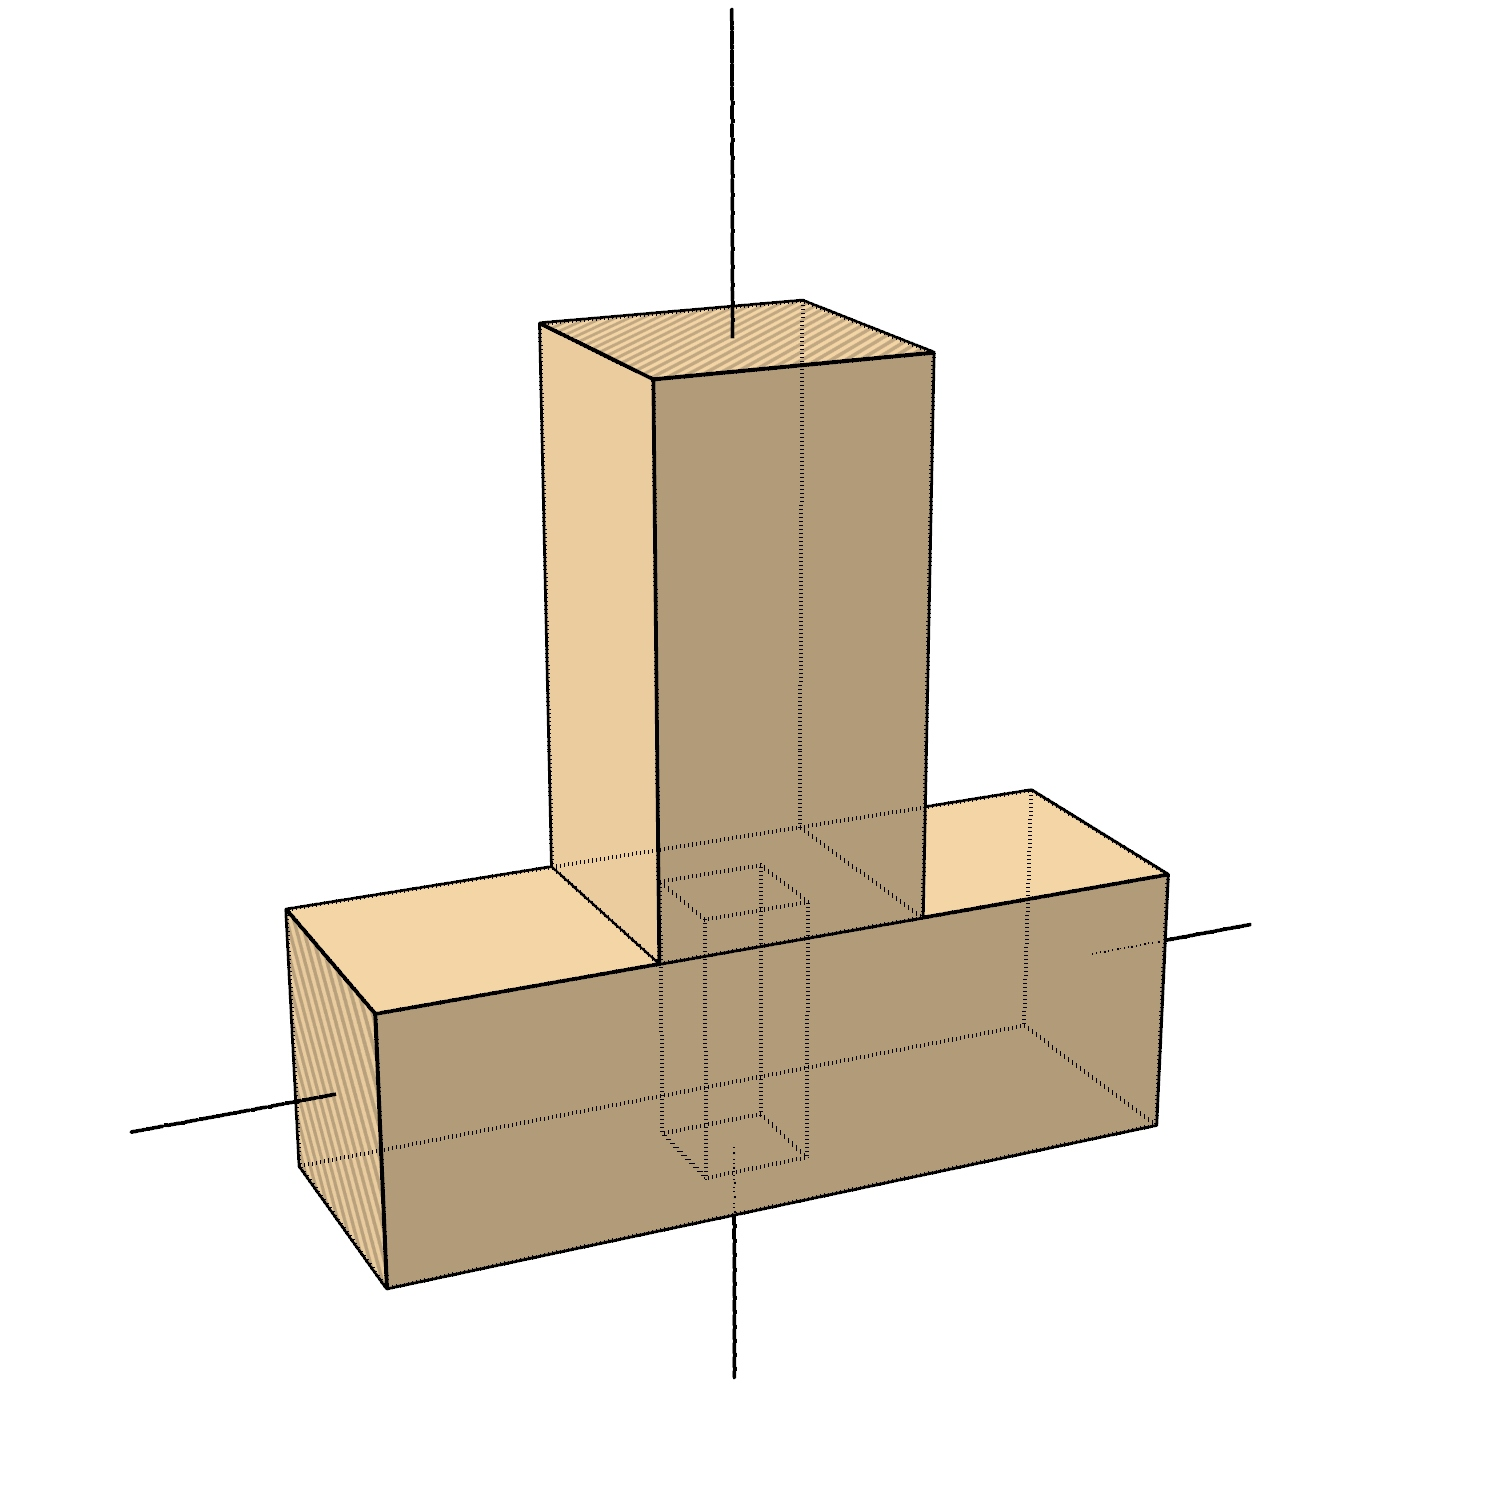
\includegraphics[width=\textwidth]{images/02/Tenon_10.jpg}
         % \caption{SubFigureCaption}
         %\label{fig:uniquesubfigurelabel}
     \end{subfigure}
     \hfill
     \begin{subfigure}[b]{0.19\textwidth}
         \centering
         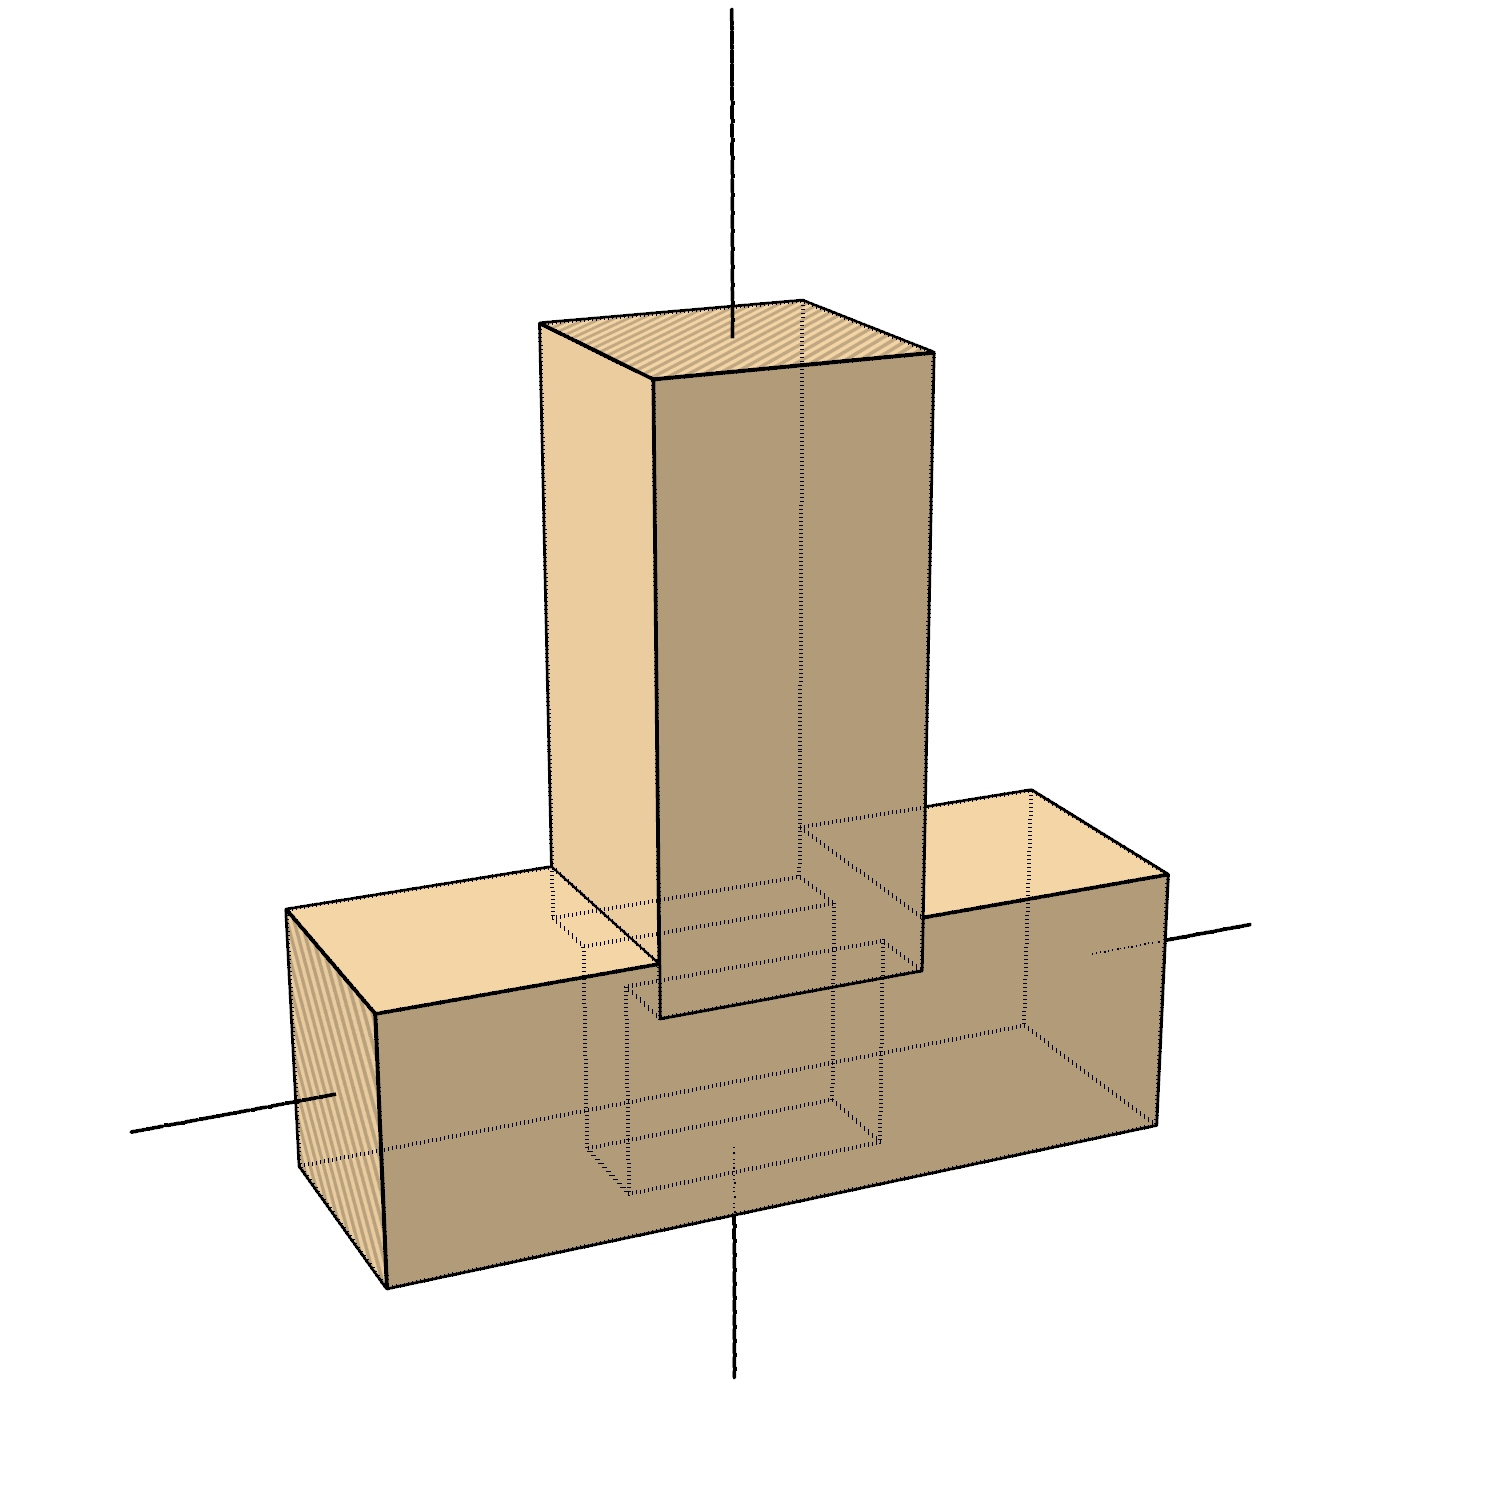
\includegraphics[width=\textwidth]{images/02/Tenon_7.jpg}
         % \caption{SubFigureCaption}
         %\label{fig:uniquesubfigurelabel}
     \end{subfigure}
     \hfill
     \begin{subfigure}[b]{0.19\textwidth}
         \centering
         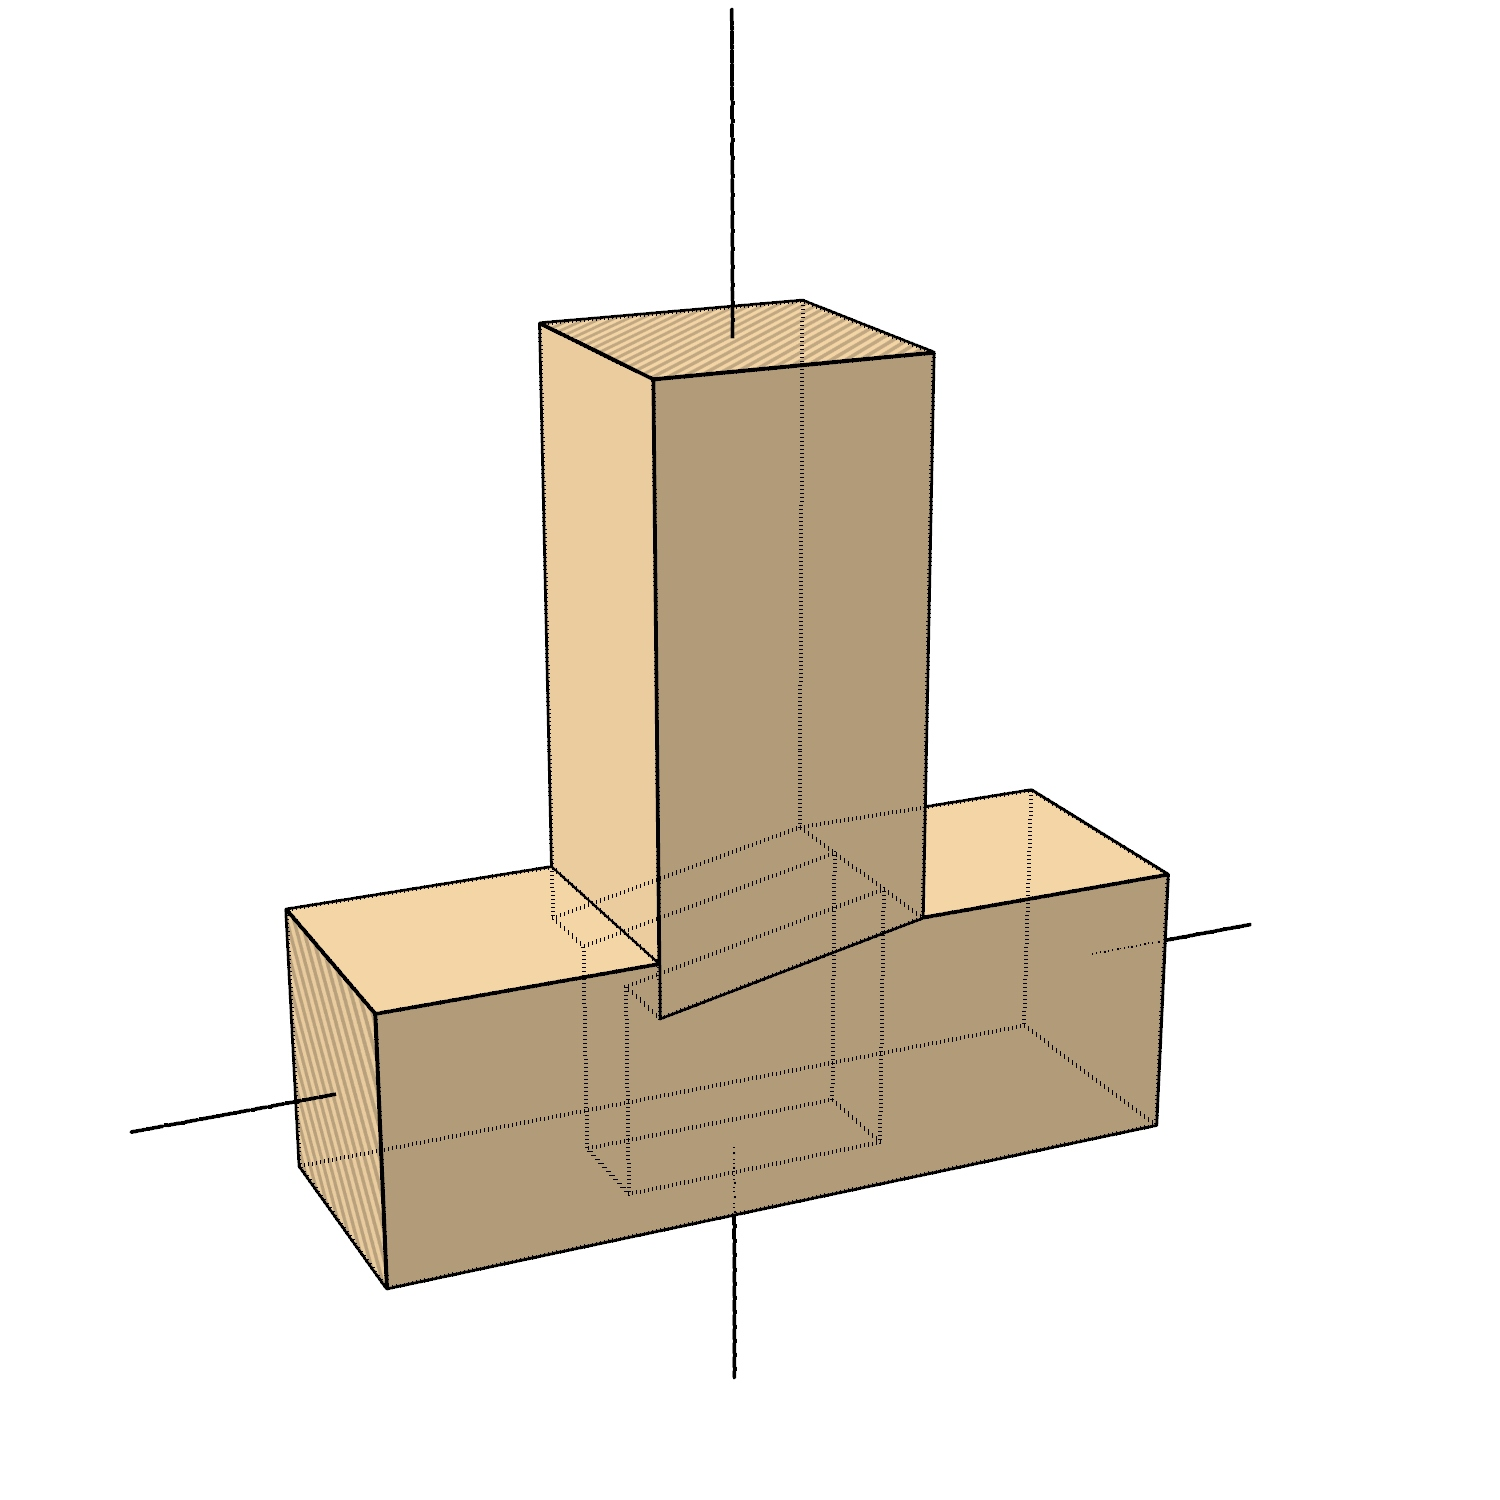
\includegraphics[width=\textwidth]{images/02/Tenon_8.jpg}
         % \caption{SubFigureCaption}
         %\label{fig:uniquesubfigurelabel}
     \end{subfigure}
        \caption{Example of a mortise and tenon joint having different topologies}
        \label{fig:mortise_tenon_different_topologies}
\end{figure}

Different ways to parametrise a joint model can result in different behaviour during size and angle adaptations. The choice of parameterization affects not only the structural behaviour of the joint but also the range of which a joint model can deform before it becomes invalid. For example, an intersection angle adaptation may result in an undercut geometry that cannot be cut with an automatic joinery machine.

Therefore it is common to consider the fabrication process and its constraints when creating a parametric joint model \parencite{vestartasDesigntoFabricationWorkflowRawSawnTimber2021}. Some joint designs are even dependent on the shape of the cutting tool. For example, the dovetail joint in Figure \ref{fig:dovetail-joint} is created by a dovetail milling cutter (Figure \ref{fig:dovetail-cutter}). In those scenarios, it is necessary to contact the fabricator for a list of possible joint feature dimensions. 

% 2 Horizontal Image  
\begin{figure}[h]
    \centering
        \begin{subfigure}[b]{0.59\textwidth}
        \centering
        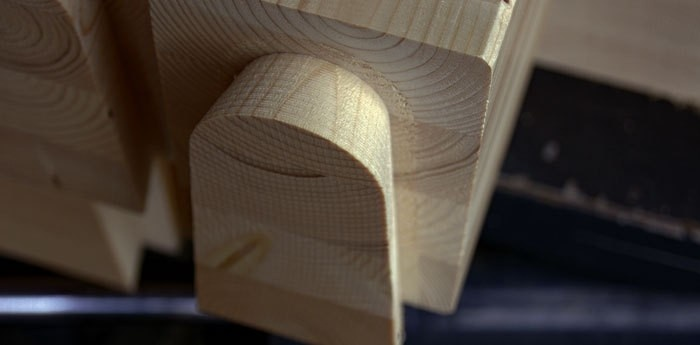
\includegraphics[width=\textwidth]{images/02/dovetailjoint.jpg}
        \caption{Example of a joint cut with a dovetail cutter}
        \label{fig:dovetail-joint}
    \end{subfigure}
    \hfill
    \begin{subfigure}[b]{0.39\textwidth}
        \centering
        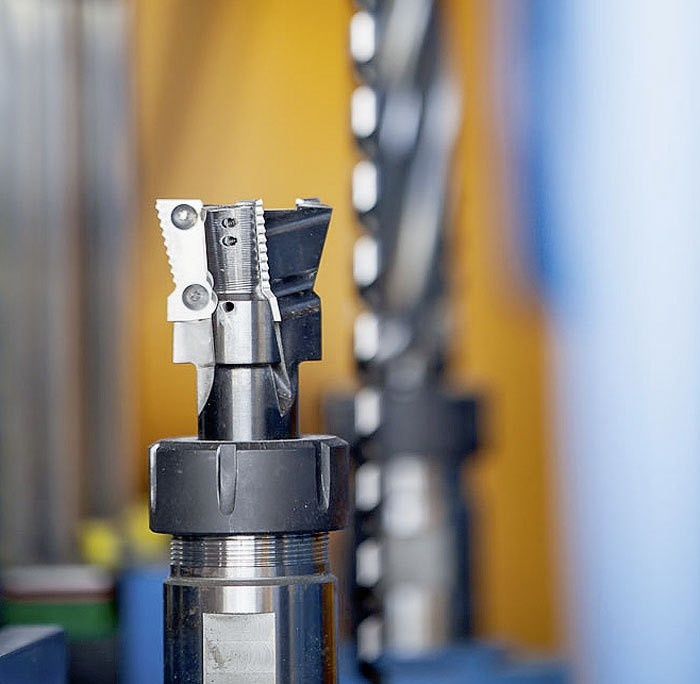
\includegraphics[trim=0mm 17mm 0mm 40mm, clip, width=\textwidth]{images/02/dovetailcutter.jpg}
        \caption{Example of a dovetail cutter}
        \label{fig:dovetail-cutter}
    \end{subfigure}
    \caption[Example of a joint cut with a shaped cutter]
    {Example of a joint cut with a shaped cutter 
        \footnotesize{(Photo by Hannes Plackner \parencite{HightechDovetails2014})}}
    \label{fig:dovetail-cutter-and-joint}
\end{figure}

Parametric joint models can be categorised according to what beam intersection topology it can adapt to. For example, side-side, side-end, and end-end types \parencite{vestartasJoinerySolverWhole2020}This grouping allows automatic determination of what parametric model can be used for a given beam intersection type. In addition, the grouping can also include the assembly direction of the beams relative to each other. Figure \ref{fig:joint_assembly_direction} shows different joints where the assembly directions is perpendicular to the beam axis (\ref{fig:assembly-direction-tee-lap} and \ref{fig:assembly-direction-cross-lap}) and parallel to the beam axis (\ref{fig:assembly-direction-mortise-tenon}).

% 3 Horizontal Image  
\begin{figure}[htb]
     \centering
     \begin{subfigure}[b]{0.32\textwidth}
         \centering
         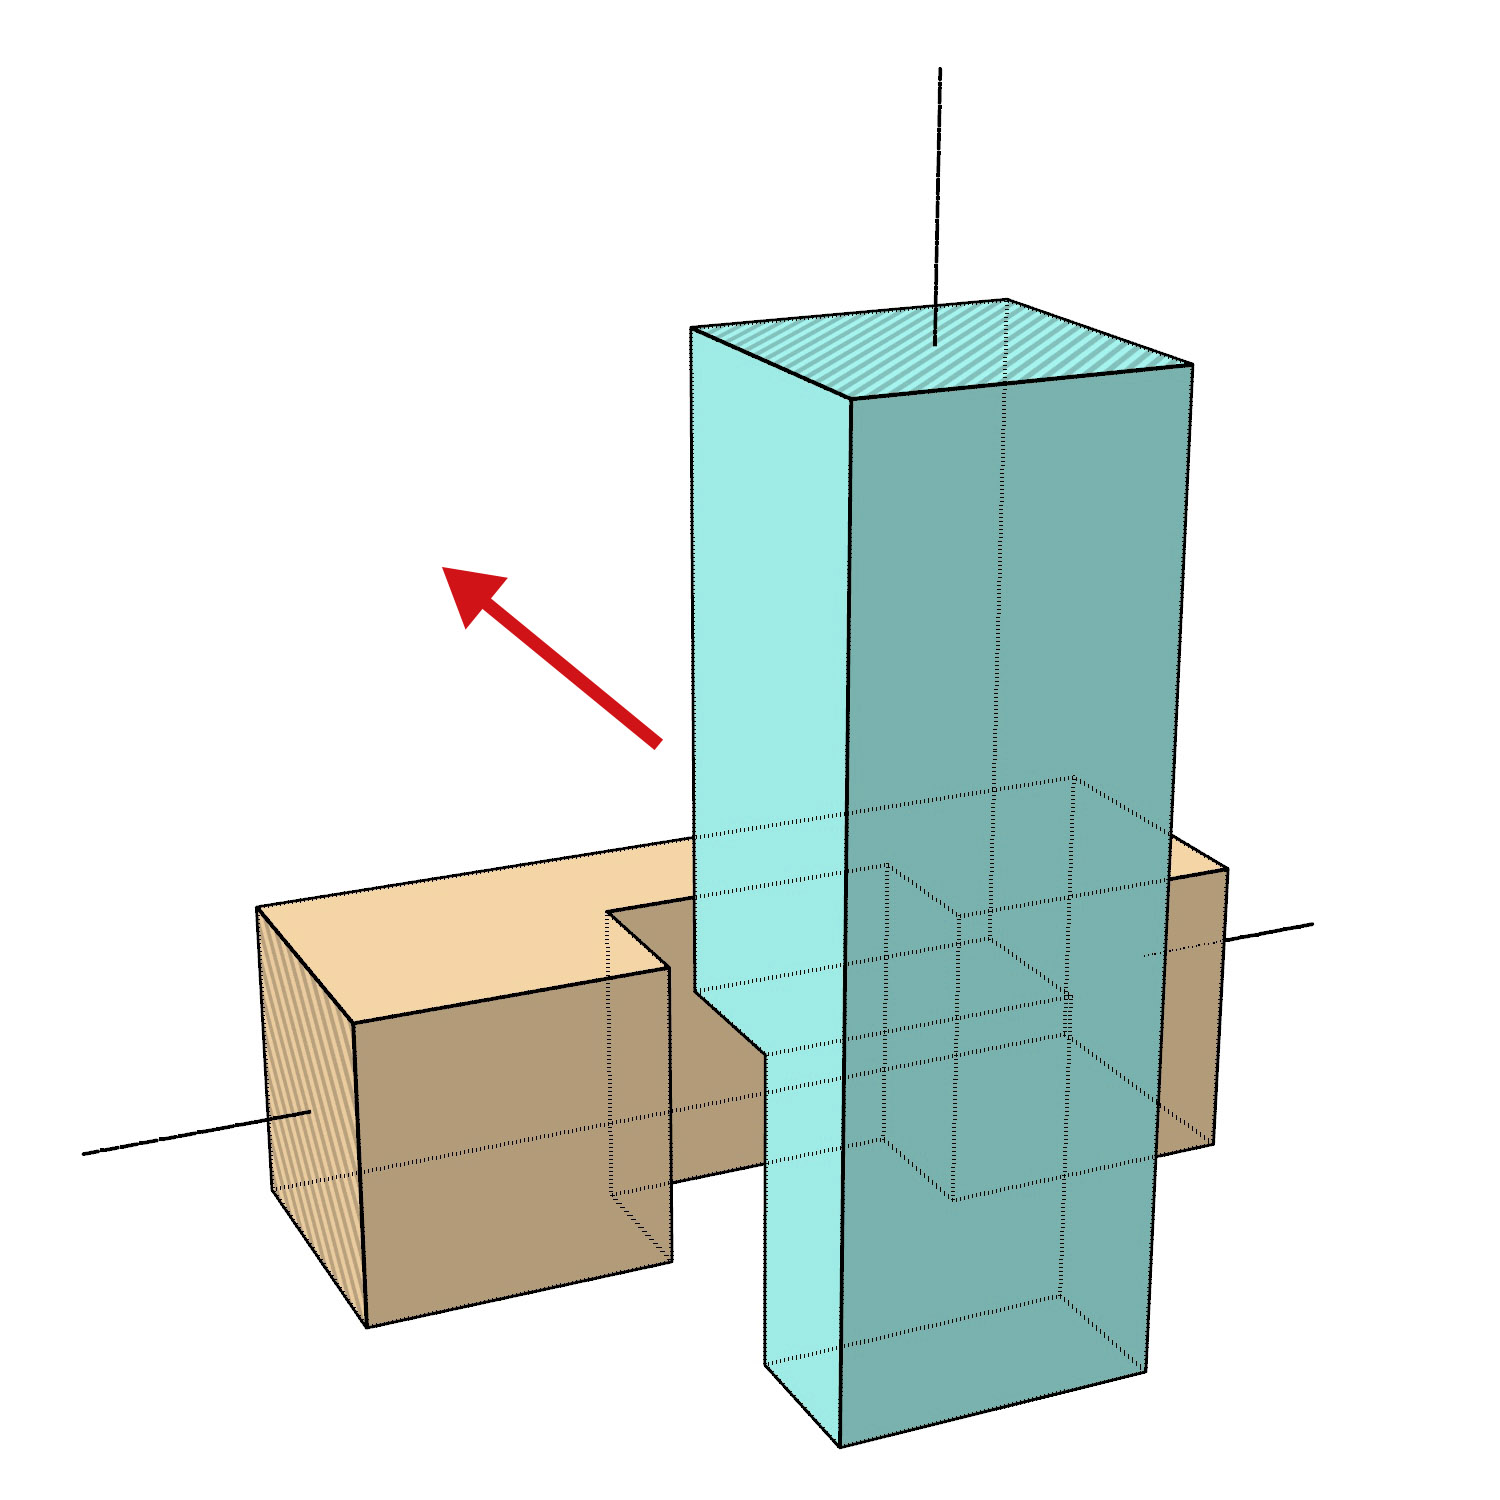
\includegraphics[width=\textwidth]{images/02/TeeLap_6_witharrows.jpg}
         \caption{Tee Lap Joint}
         \label{fig:assembly-direction-tee-lap}
     \end{subfigure}
     \hfill
     \begin{subfigure}[b]{0.32\textwidth}
         \centering
         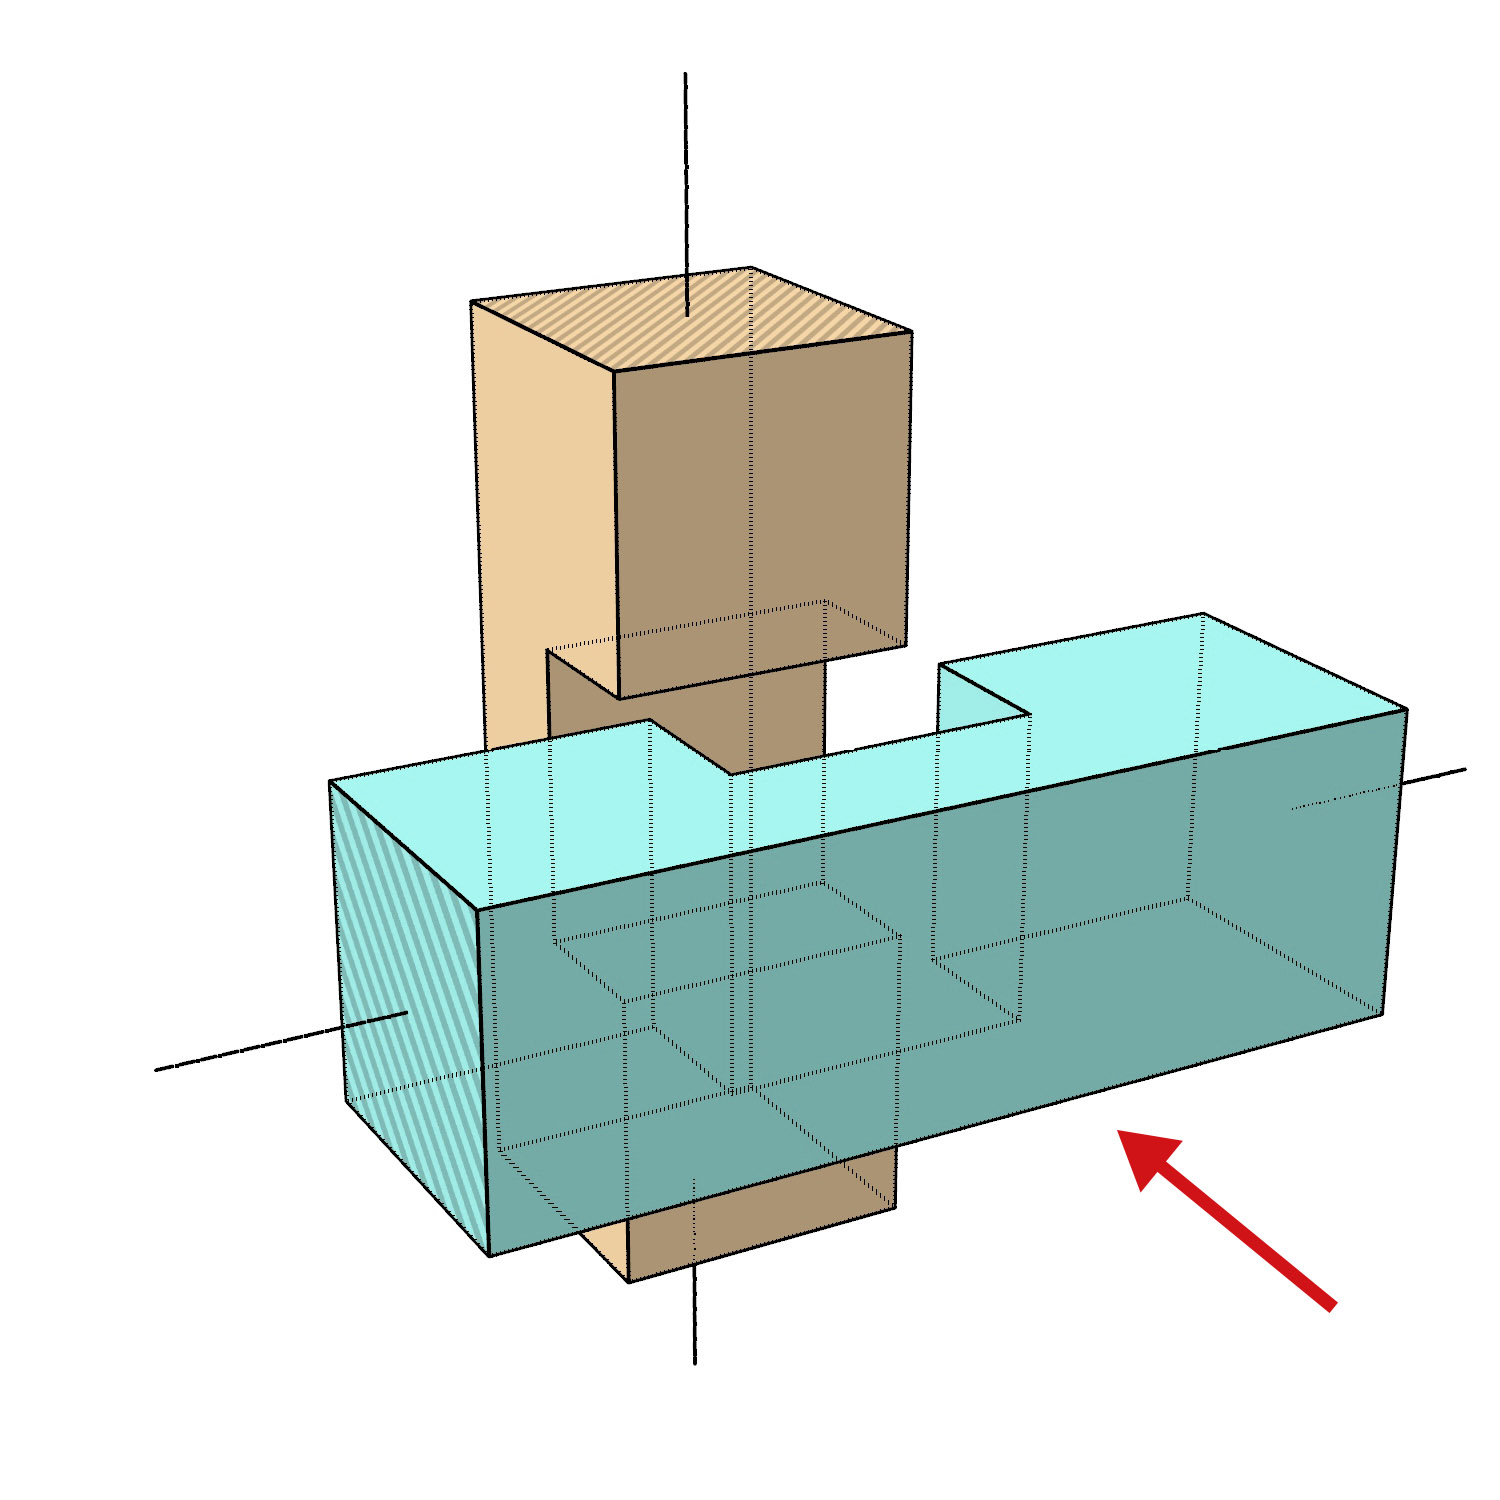
\includegraphics[width=\textwidth]{images/02/CrossLap_6_witharrows.jpg}
         \caption{Cross Lap Joint}
         \label{fig:assembly-direction-cross-lap}
     \end{subfigure}
     \hfill
     \begin{subfigure}[b]{0.32\textwidth}
         \centering
         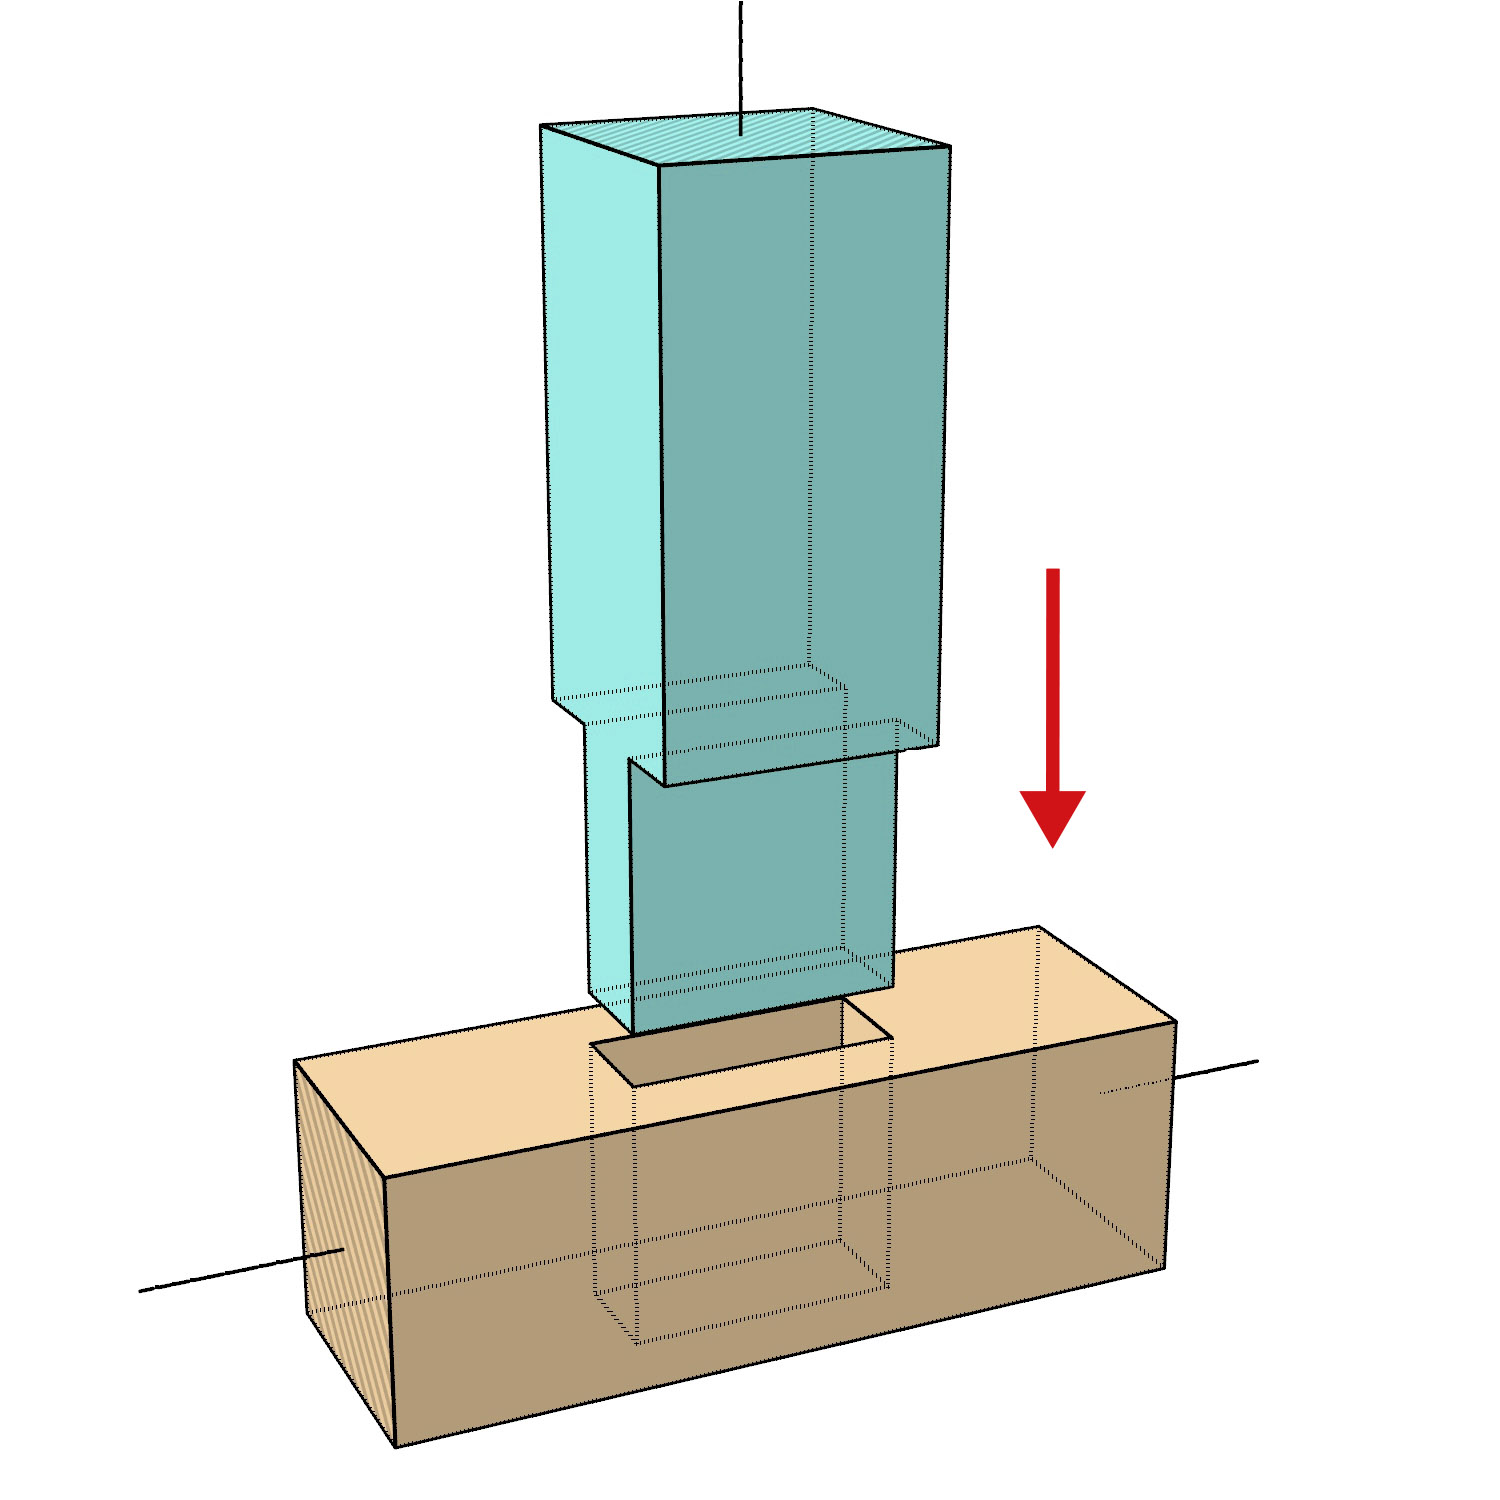
\includegraphics[width=\textwidth]{images/02/Tenon_6_witharrows.jpg}
         \caption{Mortise Tenon Joint}
         \label{fig:assembly-direction-mortise-tenon}
     \end{subfigure}
     \caption[Assembly direction of different joint types.]{Assembly direction of different joint types. Red arrow indicates the direction of movement of the light-blue piece during assembly.}
     \label{fig:joint_assembly_direction}
\end{figure}

It is worth noting that the solution space for a timber joint is large, and there are no existing approaches for evaluating all these requirements. Therefore, even though the solving process can theoretically be automatic, in practice, it often starts with the designer’s intuition and is later checked by the various design checks mentioned before. 

While the automatic modelling of timber joints is not an essential requirement for automatic assembly, it is important for a parametric design process. Even in a simple structure, there are many joints involved. The sheer number of joints makes the process tedious and prone to human error if they are modelled manually. Furthermore, the inclusion of assembly direction in a parametric joint model allows automatic design check for assemblability. It can also be used for generating the robotic assembly program, because the assembly direction defines one of the important movement targets for that specific beam. 

\subsection{User Interface for Fabrication Aware Design}
\label{subsection:challenges-user-interface-for-fabrication-aware-design}

Creating designs in a highly constrained environment is often a balance between finding interesting possibilities while pushing the design boundary. Considering the many constraints, introduced in the previous sections, that are relevant to a robotically assembled timber frame structure, it is not hard to imagine the complexity of the design process. 

The computational approach to address these highly constrained problems is to use a powerful computer to search for valid solutions that could satisfy the given boundary conditions \parencite{pottmannArchitecturalGeometryFabricationAware2013, tamFabricationawareStructuralOptimisation2018}. In theory, as long as a constraint can be committed to computer code, it can be evaluated automatically. However, this technique is only meaningful for problems where the design space and the constraints are well defined \parencite{huangFrameFabRoboticFabrication2016}. In the case of architectural design, where the design space is infinite and the aesthetics of the structure is impossible to codify, the total exclusion of a designer is not meaningful. 

The alternative is a human-computer collaborative design process, or Computer-Aided Design (CAD) in its essence, to combine the best of both agents. In this case, the Human-Computer Interface (HCI), in the form of a Graphical-User Interface (GUI), becomes critical for successful collaboration of the two \parencite{preeceInteractionDesignHumancomputer2015}. 

The primary goal for such an interface is to provide designers with real-time feedback and guidance while allowing them to explore the design space and make informed decisions \parencite{frichMappingLandscapeCreativity2019, puentesMakingGesturesDesign2015}. This involves visualising and communicating various constraints, warnings, and possible solutions through a well-designed interface that is both intuitive and user-friendly. To achieve this, the interface for designing a robotically-assemble timber structure should consider the following features: 

\begin{itemize}
	\item \textbf{Interactive 3D visualisation --} Enables navigation of the model over each assembly step for the human designer to understand temporal and spatial relationships between the beams, joints and robots.

	\item \textbf{Constraint visualisation --} Visualise constraint violations and fabrication limitations. 

	\item \textbf{Solution suggestions --} Offers ways to address constraint issues and improve the design.

	\item \textbf{Integrated robotic assembly planning --} Seamlessly incorporates assembly feasibility within the design environment.

	\item \textbf{Interactive parametric modelling workflow --} Facilitates quick iterations between different solutions when solving problems.

\end{itemize}
In summary, a user interface for fabrication-aware design should facilitate effective communication between the human designer and the computational tools, enabling a seamless and efficient design process. 

\section{Research Questions}
\label{section:research-questions}

The challenges elaborated in the previous sections have indicated the highly interdisciplinary nature of this research. It includes the field of timber frame design, digital fabrication, machine design, computer graphics and robotics. Consequently, research questions that address these challenges require an integrated approach that combines expertise from these diverse fields.

Due to the novelty of the combination of the robotic assembly and integral timber joints, the thesis will adopt an exploratory research method (details in \noseeref{chapter:methodology-and-assumptions}). In this regard, the questions are open-ended and serve as a guide for exploration. 

\begin{enumerate}
	\item \textbf{What technologies (hardware and software) are required?}

    \begin{enumerate}
    	\item What are the \textbf{robotic end effectors} needed to assemble the joints? Can they be general purpose or specific to the type of joint being assembled?
    
    	\item Is the \textbf{accuracy of a typical industrial robot }sufficient to assemble beams with joints? Is it necessary to develop \textbf{sense, alignment and compensation }methods to overcome misalignment?
    
    	\item How suitable is an industrial robotic arm for performing spatial timber assembly? How can they be designed differently if they are optimised for construction purposes? How many robots are needed to assemble a building?
    
    	\item How can \textbf{computational tools }support a robotic assembly process? Can \textbf{robotic programmes be generated automatically} based on assembly design?
    
    \end{enumerate}
    
    \item \textbf{How will architectural design workflow and detailing have to change?}

    \begin{enumerate}
    	\item Will timber frame structures and integral timber joints be designed differently to accommodate the robotic process? For example, by adding \textbf{new details }to the beams and joints to \textbf{improve ease of assembly}? Can existing timber joinery machines produce these details?
    
    	\item How will the design process be different with the added constraints of robotic assembly? How will \textbf{design validation }be performed?
    
    	\item Who are the \textbf{new domain experts responsible for an automated construction process}? How can they participate in a design workflow?
    
    \end{enumerate}
    
    \item What are the \textbf{possible implications if robots assemble timber buildings in the future?}
    
    \begin{enumerate}
    	\item Existing robots are generally not as agile as human workers. Will robotic assembly limit the \textbf{architectural and structural design possibilities}?
    
    	\item How will \textbf{humans participate} in the transition to robotic construction? How will traditional roles such as carpenters change? What are the new roles that may emerge?
    
    \end{enumerate}
\end{enumerate}

\section{Hypothesis}
\label{section:hypothesis}

This thesis is based on the hypothesis that a robotic assembly process for timber frame structures with integral timber joints is possible. The hypothesis is further broken down into several sub-hypotheses that are evaluated in the thesis:

\begin{itemize}
	\item \textbf{Sub-hypothesis 1 --} It is possible to design a robotic assembly process for spatial timber frame structures with integral timber joints. Begining with the first prototype, a novel assembly strategy using Distributed Robotic Tools (DiRT) was developed and tested on a full-scale demonstrator. The process was then refined and tested on a second and a third full-scale demonstrators. The first working hypothesis is detailed in \noseeref{subsection:exploration-1-distributed-robotic-tool-approach} and \noseeref{subsection:exploration-1-dirt-clamping-assembly-process-task-list-v1}. A later, revised hypothesis is detailed in \noseeref{subsection:exploration-3-dirt-clamping-assembly-process-task-list-v2}, the final conclusion is detailed in \noseeref{section:discussion-generalised-dirt-system}.

	\item \textbf{Sub-hypothesis 2 --} It is possible to design robotic end-effectors that can assemble integral timber joints. Over the course of the research, two types of robotic assembly tools were designed, fabricated and tested. Both of them are used for assembling lap joints, however their operating principles and capabilities are different. The first type is a robotic clamp that clamps joints together. The second type is a robotic screwdriver that pulls joints together. The combined use of both types of tools in the same structure is also tested in the third demonstrator the end of this thesis.

	\item \textbf{Sub-hypothesis 3 --} It is possible to use computational tools for the design of spatial timber frame structures with integral timber joints. Computational tools were developed to support the design of the robotic assembly process. This includes timber structure modelling tools, a robotic assembly planning tool and a user interface for designers and engineers to validate the assembly process.

	\item \textbf{Sub-hypothesis 4 --} It is possible to overcome the assembly challenges related to tolerance and alignment. Different active and passive alignment methods have been tested in this thesis. The most successful method is to chamfer the edges of the lap joints and to use the assembly tools to passively force the joints into alignment \seeref{subsection:exploration-2-clamping-joints-with-chamfered-edges}. In addition, due to need of attaching and detaching DiRT tools from the timber structure, camera-based alignment methods were tested to align the robot and the DiRT tools \seeref{subsection:exploration-4-camera-marker-alignment-correction-system}.  
	
\end{itemize}